\documentclass[11pt]{article}
\usepackage[utf8]{inputenc}\usepackage[T1]{fontenc}\usepackage{lmodern}
\usepackage[margin=1in]{geometry}
\usepackage{microtype}\setlength{\emergencystretch}{3em}
\usepackage{amsmath,amssymb,amsthm,booktabs,graphicx,array,xcolor,enumitem,caption}
\usepackage{longtable}

% Shared assets live in the original manuscript tree: one source of truth for
% every measured value, figure and table. Local files win, then the shared tree.
\makeatletter
\def\input@path{{./}{../../paper/}}
\makeatother
\graphicspath{{../../paper/figures/}}

\usepackage[round]{natbib}
% AUTO-GENERATED by paper/gen_results_macros.py. Do not edit by hand.
% Every value traces to a measured JSON artifact in this repository.
\makeatletter
\DeclareRobustCommand{\result}[1]{\@nameuse{result@#1}}
\makeatother
\expandafter\def\csname result@DebtOnlyDirect\endcsname{52}
\expandafter\def\csname result@DebtOnlyIndirect\endcsname{60}
\expandafter\def\csname result@AllClaimsDirect\endcsname{27}
\expandafter\def\csname result@AllClaimsIndirect\endcsname{47}
\expandafter\def\csname result@EquityShareDenom\endcsname{48}
\expandafter\def\csname result@DebtOnlyCV\endcsname{0.0506}
\expandafter\def\csname result@AllClaimsCV\endcsname{0.0942}
\expandafter\def\csname result@OneStepMovePct\endcsname{15}
\expandafter\def\csname result@AllClaims1947\endcsname{29}
\expandafter\def\csname result@SovUnion1947\endcsname{70}
\expandafter\def\csname result@SovHeld1947\endcsname{9}
\expandafter\def\csname result@SovObligor1947\endcsname{69}
\expandafter\def\csname result@DebtOnly1952\endcsname{52}
\expandafter\def\csname result@AllClaims1952\endcsname{28}
\expandafter\def\csname result@SovUnion1952\endcsname{52}
\expandafter\def\csname result@SovHeld1952\endcsname{9}
\expandafter\def\csname result@SovObligor1952\endcsname{51}
\expandafter\def\csname result@DebtOnly1970\endcsname{45}
\expandafter\def\csname result@AllClaims1970\endcsname{28}
\expandafter\def\csname result@SovUnion1970\endcsname{34}
\expandafter\def\csname result@SovHeld1970\endcsname{12}
\expandafter\def\csname result@SovObligor1970\endcsname{30}
\expandafter\def\csname result@DebtOnly1990\endcsname{46}
\expandafter\def\csname result@AllClaims1990\endcsname{35}
\expandafter\def\csname result@SovUnion1990\endcsname{56}
\expandafter\def\csname result@SovHeld1990\endcsname{25}
\expandafter\def\csname result@SovObligor1990\endcsname{36}
\expandafter\def\csname result@DebtOnly2000\endcsname{47}
\expandafter\def\csname result@AllClaims2000\endcsname{27}
\expandafter\def\csname result@SovUnion2000\endcsname{56}
\expandafter\def\csname result@SovHeld2000\endcsname{32}
\expandafter\def\csname result@SovObligor2000\endcsname{30}
\expandafter\def\csname result@DebtOnly2008\endcsname{50}
\expandafter\def\csname result@AllClaims2008\endcsname{38}
\expandafter\def\csname result@SovUnion2008\endcsname{56}
\expandafter\def\csname result@SovHeld2008\endcsname{30}
\expandafter\def\csname result@SovObligor2008\endcsname{29}
\expandafter\def\csname result@DebtOnly2020\endcsname{50}
\expandafter\def\csname result@AllClaims2020\endcsname{29}
\expandafter\def\csname result@SovUnion2020\endcsname{78}
\expandafter\def\csname result@SovHeld2020\endcsname{39}
\expandafter\def\csname result@SovObligor2020\endcsname{52}
\expandafter\def\csname result@DebtOnly2025\endcsname{52}
\expandafter\def\csname result@AllClaims2025\endcsname{27}
\expandafter\def\csname result@SovUnion2025\endcsname{79}
\expandafter\def\csname result@SovHeld2025\endcsname{32}
\expandafter\def\csname result@SovObligor2025\endcsname{55}
\expandafter\def\csname result@AllClaimsSeriesLow\endcsname{25}
\expandafter\def\csname result@AllClaimsSeriesHigh\endcsname{38}
\expandafter\def\csname result@DebtOnlySeriesLow\endcsname{44}
\expandafter\def\csname result@DebtOnlySeriesHigh\endcsname{52}
\expandafter\def\csname result@OneStepMoveAllClaimsPct\endcsname{76}
\expandafter\def\csname result@MultifamilyZeroMovePct\endcsname{4.4}
\expandafter\def\csname result@CommercialRentMovePct\endcsname{7.1}
\expandafter\def\csname result@StructIndirect\endcsname{45}
\expandafter\def\csname result@StructNoPools\endcsname{59}
\expandafter\def\csname result@StructCommercial\endcsname{74}
\expandafter\def\csname result@StructObligorExcluded\endcsname{32}
\expandafter\def\csname result@MeasurementMaxMovePct\endcsname{1.29}
\expandafter\def\csname result@MeasurementMaxMoveRounded\endcsname{1}
\expandafter\def\csname result@AgreedRangeLow\endcsname{78}
\expandafter\def\csname result@AgreedRangeHigh\endcsname{80}
\expandafter\def\csname result@OverlapBn\endcsname{3,226.4}
\expandafter\def\csname result@AIFederalShare\endcsname{1.0}
\expandafter\def\csname result@AIFederalShareRounded\endcsname{1}
\expandafter\def\csname result@AIFederalShareLow\endcsname{1.0}
\expandafter\def\csname result@AIFederalShareHigh\endcsname{1.0}
\expandafter\def\csname result@AIEquityScale\endcsname{20}
\expandafter\def\csname result@HolderGap\endcsname{78}
\expandafter\def\csname result@QOnePerDollar\endcsname{4.15}
\expandafter\def\csname result@QTwoPerDollar\endcsname{1.41}
\expandafter\def\csname result@QTopPerDollar\endcsname{0.65}
\expandafter\def\csname result@QOnePerDollarOwnSurvey\endcsname{4.14}
\expandafter\def\csname result@QAggMultiplier\endcsname{1.4859}
\expandafter\def\csname result@QOneLevel\endcsname{6.16}
\expandafter\def\csname result@QTwoLevel\endcsname{2.10}
\expandafter\def\csname result@QTopLevel\endcsname{0.97}
\expandafter\def\csname result@QTopWageShare\endcsname{51}
\expandafter\def\csname result@SovUnionTroughYear\endcsname{1965}
\expandafter\def\csname result@SovUnionTrough\endcsname{30.8}
\expandafter\def\csname result@SovUnionRiseFromTrough\endcsname{2.6}
\expandafter\def\csname result@SovUnionRiseFrom1947\endcsname{1.14}
\expandafter\def\csname result@QuintDenomDivergence\endcsname{9.6}
\expandafter\def\csname result@QOneAgreement\endcsname{0.31}
\expandafter\def\csname result@QTopClaimShare\endcsname{34}
\expandafter\def\csname result@SovereignUnion\endcsname{79.5}
\expandafter\def\csname result@SovereignCreditor\endcsname{32}
\expandafter\def\csname result@SovereignDebtor\endcsname{56}
\expandafter\def\csname result@WageBackedStockBn\endcsname{39,957.1}
\expandafter\def\csname result@SovereignUnionCoverage\endcsname{79}
\expandafter\def\csname result@SovereignCreditorCoverage\endcsname{32}
\expandafter\def\csname result@SovereignDebtorCoverage\endcsname{55}
\expandafter\def\csname result@AllClaimsDirectCoverage\endcsname{27}
\expandafter\def\csname result@AllClaimsIndirectCoverage\endcsname{47}
\expandafter\def\csname result@DebtOnlyIndirectCoverage\endcsname{60}
\expandafter\def\csname result@GainsAGILow\endcsname{6.2}
\expandafter\def\csname result@GainsAGIHigh\endcsname{15.4}
\expandafter\def\csname result@ReceiptsShareLow\endcsname{0.6339}
\expandafter\def\csname result@ReceiptsShareHigh\endcsname{0.6528}
\expandafter\def\csname result@ReceiptsPctLow\endcsname{63}
\expandafter\def\csname result@ReceiptsPctHigh\endcsname{65}
\expandafter\def\csname result@RetainedWageShare\endcsname{0.5683}
\expandafter\def\csname result@RhoReemploy\endcsname{0.661}
\expandafter\def\csname result@OmegaRetention\endcsname{0.8598}
\expandafter\def\csname result@RequiredLow\endcsname{11.0}
\expandafter\def\csname result@RequiredHigh\endcsname{13.7}
\expandafter\def\csname result@TauKBarkai\endcsname{8.5}
\expandafter\def\csname result@TauKBarkaiLow\endcsname{7.2}
\expandafter\def\csname result@TauKBarkaiHigh\endcsname{9.6}
\expandafter\def\csname result@TauKKN\endcsname{1.5}
\expandafter\def\csname result@TauKPassLow\endcsname{0.0}
\expandafter\def\csname result@TauKPassHigh\endcsname{0}
\expandafter\def\csname result@TauKOperativeOld\endcsname{7.1}
\expandafter\def\csname result@ShareholderLayer\endcsname{0.0386}
\expandafter\def\csname result@ThetaTaxable\endcsname{27}
\expandafter\def\csname result@ThetaUntaxable\endcsname{73}
\expandafter\def\csname result@DeferralCentral\endcsname{0.601}
\expandafter\def\csname result@GainsUntaxedAtDeath\endcsname{46.9}
\expandafter\def\csname result@InterestSheltered\endcsname{32.8}
\expandafter\def\csname result@TaxableHolderInterestRate\endcsname{27.4}
\expandafter\def\csname result@CBOFullyTaxableEquity\endcsname{57.2}
\expandafter\def\csname result@CBODebtFinancedETR\endcsname{6}
\expandafter\def\csname result@BondsRestOfWorld\endcsname{28.7}
\expandafter\def\csname result@BondsHouseholdDirect\endcsname{1.1}
\expandafter\def\csname result@RequiredEasy\endcsname{11.0}
\expandafter\def\csname result@RequiredHard\endcsname{13.7}
\expandafter\def\csname result@TauKAnalyticMax\endcsname{11.5}
\expandafter\def\csname result@CRSTheta\endcsname{45.5}
\expandafter\def\csname result@TauKCRSCentral\endcsname{10.2}
\expandafter\def\csname result@TauKCRSPassShare\endcsname{22}
\expandafter\def\csname result@TauKCRSAnalyticMax\endcsname{14.2}
\expandafter\def\csname result@TauKCRSKN\endcsname{3.2}
\expandafter\def\csname result@CRSTextFigure\endcsname{3.1}
\expandafter\def\csname result@CRSBandLow\endcsname{4.5}
\expandafter\def\csname result@CRSBandHigh\endcsname{8.5}
\expandafter\def\csname result@CRSRescaledLow\endcsname{2.7}
\expandafter\def\csname result@CRSRescaledHigh\endcsname{5.1}
\expandafter\def\csname result@ShareholderLayerPct\endcsname{3.9}
\expandafter\def\csname result@SwingDeferral\endcsname{0.0159}
\expandafter\def\csname result@SwingStateCIT\endcsname{0.0133}
\expandafter\def\csname result@SwingShifted\endcsname{0.0025}
\expandafter\def\csname result@SwingShareholderRate\endcsname{0.0115}
\expandafter\def\csname result@SwingDebtShare\endcsname{0.0063}
\expandafter\def\csname result@SwingBondRate\endcsname{0.0042}
\expandafter\def\csname result@SwingTheta\endcsname{0.0037}
\expandafter\def\csname result@DebtShareLow\endcsname{14.1}
\expandafter\def\csname result@DebtShareHigh\endcsname{25.9}
\expandafter\def\csname result@BondRateLow\endcsname{14.3}
\expandafter\def\csname result@BondRateHigh\endcsname{17.5}
\expandafter\def\csname result@DeferralLow\endcsname{0.412}
\expandafter\def\csname result@DeferralHigh\endcsname{0.790}
\expandafter\def\csname result@ThetaTaxableLow\endcsname{24}
\expandafter\def\csname result@ThetaTaxableHigh\endcsname{28}
\expandafter\def\csname result@FedCIT\endcsname{21}
\expandafter\def\csname result@FDDEIRate\endcsname{14.0}
\expandafter\def\csname result@CFCRate\endcsname{12.6}
\expandafter\def\csname result@RentBarkai\endcsname{0.351}
\expandafter\def\csname result@ShiftedShare\endcsname{48}
\expandafter\def\csname result@WageBillBn\endcsname{13,365.2}
\expandafter\def\csname result@FedReceiptsBn\endcsname{5,980.6}
\expandafter\def\csname result@PlausChecks\endcsname{59}
\expandafter\def\csname result@PlausViolations\endcsname{4}
\expandafter\def\csname result@RepTwoScored\endcsname{127}
\expandafter\def\csname result@RepTwoSealed\endcsname{79}
\expandafter\def\csname result@RepTwoTolerance\endcsname{28}
\expandafter\def\csname result@RepTwoFivePct\endcsname{45}
\expandafter\def\csname result@RepTwoMismatch\endcsname{34}
\expandafter\def\csname result@RepThreeSealed\endcsname{32}
\expandafter\def\csname result@RepThreeRounding\endcsname{30}
\expandafter\def\csname result@RepThreeMismatch\endcsname{0}
\expandafter\def\csname result@ExcludedInstitutions\endcsname{24}
\expandafter\def\csname result@ExcludedAssetsBn\endcsname{263.2}
\expandafter\def\csname result@SystemAssetsBn\endcsname{29,012.5}
\expandafter\def\csname result@BaselineBreaches\endcsname{29}
\expandafter\def\csname result@BaselinePctAssets\endcsname{0.029}
\expandafter\def\csname result@TerminalLossTen\endcsname{85.168}
\expandafter\def\csname result@FedShareTenNarrowLow\endcsname{79}
\expandafter\def\csname result@FedShareTenNarrowHigh\endcsname{87}
\expandafter\def\csname result@FedShareTenConsLow\endcsname{88}
\expandafter\def\csname result@FedShareTenConsHigh\endcsname{91}
\expandafter\def\csname result@FedShareFiftyNarrowLow\endcsname{86}
\expandafter\def\csname result@FedShareFiftyNarrowHigh\endcsname{93}
\expandafter\def\csname result@FedShareSeventyFiveNarrowHigh\endcsname{90}
\expandafter\def\csname result@FedFirstRoundTenLow\endcsname{179}
\expandafter\def\csname result@FedFirstRoundTenHigh\endcsname{223}
\expandafter\def\csname result@PrivateFirstRoundTenLow\endcsname{32}
\expandafter\def\csname result@PrivateFirstRoundTenHigh\endcsname{52}
\expandafter\def\csname result@OASDILossTenLow\endcsname{54}
\expandafter\def\csname result@OASDILossTenHigh\endcsname{73}
\expandafter\def\csname result@HILossTenLow\endcsname{17}
\expandafter\def\csname result@HILossTenHigh\endcsname{21}
\expandafter\def\csname result@UnenhancedLow\endcsname{39}
\expandafter\def\csname result@UnenhancedHigh\endcsname{53}
\expandafter\def\csname result@PrivateCoverLow\endcsname{6}
\expandafter\def\csname result@PrivateCoverHigh\endcsname{11}
\expandafter\def\csname result@AgencyCapitalBn\endcsname{179.4}
\expandafter\def\csname result@MaxRetainedAgencyLossBn\endcsname{109.0}
\expandafter\def\csname result@TreasuryDrawBn\endcsname{0}
\expandafter\def\csname result@QOneRunway\endcsname{1.26}
\expandafter\def\csname result@QOneUnderOne\endcsname{47.7}
\expandafter\def\csname result@QTwoRunway\endcsname{0.84}
\expandafter\def\csname result@QTwoUnderOne\endcsname{55.1}
\expandafter\def\csname result@QThreeRunway\endcsname{1.09}
\expandafter\def\csname result@QThreeUnderOne\endcsname{49.7}
\expandafter\def\csname result@QFourRunway\endcsname{1.40}
\expandafter\def\csname result@QFourUnderOne\endcsname{43.2}
\expandafter\def\csname result@QFiveRunway\endcsname{1.81}
\expandafter\def\csname result@QFiveUnderOne\endcsname{36.4}
\expandafter\def\csname result@PayGapSurvivingLow\endcsname{1.7}
\expandafter\def\csname result@PayGapSurvivingHigh\endcsname{7.0}
\expandafter\def\csname result@PayCells\endcsname{4}
\expandafter\def\csname result@AttritionStudentLow\endcsname{35}
\expandafter\def\csname result@AttritionStudentHigh\endcsname{66}
\expandafter\def\csname result@AttritionAutoLow\endcsname{-7}
\expandafter\def\csname result@AttritionAutoHigh\endcsname{15}
\expandafter\def\csname result@AttritionMortgageLow\endcsname{19}
\expandafter\def\csname result@AttritionMortgageHigh\endcsname{32}
\expandafter\def\csname result@NInstitutions\endcsname{8,588}
\expandafter\def\csname result@NBanks\endcsname{4,296}
\expandafter\def\csname result@NCreditUnions\endcsname{4,292}
\expandafter\def\csname result@SysLossTen\endcsname{205}
\expandafter\def\csname result@SysFirstTen\endcsname{23}
\expandafter\def\csname result@SysSecondTen\endcsname{182}
\expandafter\def\csname result@SecondRoundShareTen\endcsname{89}
\expandafter\def\csname result@BreachTenN\endcsname{54}
\expandafter\def\csname result@BreachTenAssets\endcsname{0.04}
\expandafter\def\csname result@BreachTwentyFiveN\endcsname{246}
\expandafter\def\csname result@BreachTwentyFiveAssets\endcsname{4.02}
\expandafter\def\csname result@BreachTwentyFiveAssetsEarnings\endcsname{1.55}
\expandafter\def\csname result@BreachFiftyN\endcsname{1,448}
\expandafter\def\csname result@BreachFiftyAssets\endcsname{28.2}
\expandafter\def\csname result@BreachFiftyAssetsEarnings\endcsname{9.9}
\expandafter\def\csname result@SysLossFifty\endcsname{1,262}
\expandafter\def\csname result@CardHeavyTwentyFiveInst\endcsname{38.89}
\expandafter\def\csname result@CardHeavyTwentyFiveAssets\endcsname{84.40}
\expandafter\def\csname result@CardHeavyFiftyInst\endcsname{77.78}
\expandafter\def\csname result@CreditUnionTenInst\endcsname{1.12}
\expandafter\def\csname result@MortgageLenderTwentyFiveInst\endcsname{0.14}
\expandafter\def\csname result@ReliefRemovedTen\endcsname{9.61}
\expandafter\def\csname result@ReliefRemovedTwentyFive\endcsname{8.91}
\expandafter\def\csname result@ReliefRemovedFifty\endcsname{7.59}
\expandafter\def\csname result@ReliefRemovedTenBn\endcsname{19.7}
\expandafter\def\csname result@ReliefAssetsBeforeTwentyFive\endcsname{4.02}
\expandafter\def\csname result@ReliefAssetsAfterTwentyFive\endcsname{1.48}
\expandafter\def\csname result@ReliefStoppedTwentyFive\endcsname{123}
\expandafter\def\csname result@WageInsuranceCost\endcsname{314}
\expandafter\def\csname result@WageInsuranceRemoved\endcsname{12.9}
\expandafter\def\csname result@StateLocalWageLinkedBn\endcsname{424.1}
\expandafter\def\csname result@StateLocalWageLinkedShare\endcsname{16}
\expandafter\def\csname result@PensionHoldingsBn\endcsname{444.6}
\expandafter\def\csname result@InsurerHoldingsBn\endcsname{820.6}
\expandafter\def\csname result@OtherFinancialHoldingsBn\endcsname{6,186.9}
\expandafter\def\csname result@AIBankCommitmentsBn\endcsname{450}
\expandafter\def\csname result@TopOnePctEquity\endcsname{50.9}
\expandafter\def\csname result@BottomHalfEquity\endcsname{0.6}
\expandafter\def\csname result@MPCWealth\endcsname{3.2}
\expandafter\def\csname result@FilerCapexBn\endcsname{490.9}
\expandafter\def\csname result@FilerOCFBn\endcsname{659.1}
\expandafter\def\csname result@SelfFunding\endcsname{1.34}
\expandafter\def\csname result@DebtFinancedShare\endcsname{6.5}
\expandafter\def\csname result@OnBalanceSheetAIDebtBn\endcsname{458.4}
\expandafter\def\csname result@FlipToBetweenBn\endcsname{66.1}
\expandafter\def\csname result@FlipToBetweenShare\endcsname{14.7}
\expandafter\def\csname result@FlipToDebtLedBn\endcsname{213.3}
\expandafter\def\csname result@FlipToDebtLedShare\endcsname{47.4}
\expandafter\def\csname result@AIDrawnBn\endcsname{162}
\expandafter\def\csname result@BustWageLow\endcsname{0.12}
\expandafter\def\csname result@BustWageHigh\endcsname{0.84}
\expandafter\def\csname result@BustRatioLow\endcsname{12}
\expandafter\def\csname result@BustRatioHigh\endcsname{80}
\expandafter\def\csname result@BustCreditLow\endcsname{0.8}
\expandafter\def\csname result@BustCreditHigh\endcsname{5.4}
\expandafter\def\csname result@BustReceiptsLow\endcsname{569}
\expandafter\def\csname result@BustReceiptsHigh\endcsname{955}
\expandafter\def\csname result@EquityLedReceiptsPct\endcsname{9.5}
\expandafter\def\csname result@EquityLedCorpPct\endcsname{35.1}
\expandafter\def\csname result@CreditLedReceiptsPct\endcsname{16.0}
\expandafter\def\csname result@CreditLedCorpPct\endcsname{53.4}
\expandafter\def\csname result@BustGDPLow\endcsname{0.34}
\expandafter\def\csname result@BustGDPHigh\endcsname{1.69}
\expandafter\def\csname result@FedPayoffFails\endcsname{-0.013}
\expandafter\def\csname result@FedPayoffPartial\endcsname{-0.166}
\expandafter\def\csname result@FedPayoffSuccess\endcsname{-0.311}
\expandafter\def\csname result@HouseholdPayoffSuccess\endcsname{0.324}
\expandafter\def\csname result@BanksAISide\endcsname{3.2}
\expandafter\def\csname result@HouseholdsAISide\endcsname{38.4}
\expandafter\def\csname result@HHBottomQuartileAffected\endcsname{85}
\expandafter\def\csname result@HHTopOnePctAffected\endcsname{24}
\expandafter\def\csname result@HHDebtAffected\endcsname{59}
\expandafter\def\csname result@HHRestoreFive\endcsname{8}
\expandafter\def\csname result@HHRestoreTen\endcsname{17}
\expandafter\def\csname result@HHEquityOutsideHouseholds\endcsname{47}
\expandafter\def\csname result@HHEquityInRetirement\endcsname{25}
\expandafter\def\csname result@AISideTotalBn\endcsname{14,857.4}
\expandafter\def\csname result@StakeForTenPctBn\endcsname{1,486}
\expandafter\def\csname result@GapClosedAtTenPct\endcsname{11}
\expandafter\def\csname result@StakeVersusAgencyCapital\endcsname{8}
\expandafter\def\csname result@BreakEvenALow\endcsname{12.5}
\expandafter\def\csname result@BreakEvenAHigh\endcsname{30.1}
\expandafter\def\csname result@BreakEvenBLow\endcsname{18.2}
\expandafter\def\csname result@BreakEvenBHigh\endcsname{65.0}
\expandafter\def\csname result@EMBaseline\endcsname{376.7}
\expandafter\def\csname result@EMIncrementLow\endcsname{10.1}
\expandafter\def\csname result@EMIncrementHigh\endcsname{12.6}
\expandafter\def\csname result@ReserveIncrementLow\endcsname{5.6}
\expandafter\def\csname result@ReserveIncrementHigh\endcsname{7.0}
\expandafter\def\csname result@EMRatio\endcsname{1.8}
\expandafter\def\csname result@PrimeAgeNonemp\endcsname{19.31}
\expandafter\def\csname result@PrimeAgeMax\endcsname{24.71}
\expandafter\def\csname result@DisplacementFlow\endcsname{0.00679}
\expandafter\def\csname result@GradUnemployment\endcsname{5.6}
\expandafter\def\csname result@GradUnderemployment\endcsname{42.0}
\expandafter\def\csname result@AutoDelinquency\endcsname{5.49}
\expandafter\def\csname result@OASDIDepletion\endcsname{2034 Q3}
\expandafter\def\csname result@GCentral\endcsname{0.66}
\expandafter\def\csname result@GLow\endcsname{0.35}
\expandafter\def\csname result@GHigh\endcsname{0.90}
\expandafter\def\csname result@RequiredPTEasy\endcsname{17}
\expandafter\def\csname result@RequiredPTHarder\endcsname{21}
\expandafter\def\csname result@GWithPrice\endcsname{0.51}
\expandafter\def\csname result@RequiredPriceEasy\endcsname{22}
\expandafter\def\csname result@RequiredPriceHarder\endcsname{27}
\expandafter\def\csname result@PriceThrough\endcsname{30}
\expandafter\def\csname result@CapitalCostShare\endcsname{50}
\expandafter\def\csname result@CapexDomesticLabor\endcsname{19}
\expandafter\def\csname result@CapexImported\endcsname{47}
\expandafter\def\csname result@CapexDomesticSurplus\endcsname{32}
\expandafter\def\csname result@TransitionPositiveYear\endcsname{4}
\expandafter\def\csname result@TransitionYearOne\endcsname{0.11}
\expandafter\def\csname result@TransitionYearFive\endcsname{0.036}
\expandafter\def\csname result@TransitionYearTwentyFive\endcsname{0.010}
\expandafter\def\csname result@TransitionGrowthRate\endcsname{20}
\expandafter\def\csname result@ReliefNoFeedbackTen\endcsname{9.6}
\expandafter\def\csname result@ReliefFeedbackTen\endcsname{62.2}
\expandafter\def\csname result@ReliefCostTen\endcsname{318}
\expandafter\def\csname result@ReliefAssetsBeforeTen\endcsname{0.04}
\expandafter\def\csname result@ReliefAssetsNoFeedbackTen\endcsname{0.03}
\expandafter\def\csname result@ReliefAssetsFeedbackTen\endcsname{0.03}
\expandafter\def\csname result@ReliefNoFeedbackTwentyFive\endcsname{8.9}
\expandafter\def\csname result@ReliefFeedbackTwentyFive\endcsname{64.5}
\expandafter\def\csname result@ReliefCostTwentyFive\endcsname{947}
\expandafter\def\csname result@ReliefAssetsNoFeedbackTwentyFive\endcsname{1.48}
\expandafter\def\csname result@ReliefAssetsFeedbackTwentyFive\endcsname{0.05}
\expandafter\def\csname result@ReliefNoFeedbackFifty\endcsname{7.6}
\expandafter\def\csname result@ReliefFeedbackFifty\endcsname{69.2}
\expandafter\def\csname result@ReliefCostFifty\endcsname{2,799}
\expandafter\def\csname result@ReliefAssetsBeforeFifty\endcsname{28.20}
\expandafter\def\csname result@ReliefAssetsNoFeedbackFifty\endcsname{25.35}
\expandafter\def\csname result@ReliefAssetsFeedbackFifty\endcsname{1.26}
\expandafter\def\csname result@CardHeavyReliefNoFeedback\endcsname{31.8}
\expandafter\def\csname result@CardHeavyReliefFeedback\endcsname{0.4}
\expandafter\def\csname result@CUReliefNoFeedbackFifty\endcsname{30.5}
\expandafter\def\csname result@CUReliefFeedbackFifty\endcsname{0.5}
\expandafter\def\csname result@ClosingMultipleLow\endcsname{1.29}
\expandafter\def\csname result@ClosingMultipleHigh\endcsname{1.61}
\expandafter\def\csname result@BustFallLow\endcsname{569}
\expandafter\def\csname result@BustFallHigh\endcsname{955}
\expandafter\def\csname result@BustAtRiskIncreaseLow\endcsname{167}
\expandafter\def\csname result@BustAtRiskIncreaseHigh\endcsname{586}
\expandafter\def\csname result@PassShareOursEasy\endcsname{0.00}
\expandafter\def\csname result@PassShareOursHard\endcsname{0.00}
\expandafter\def\csname result@PassShareCRSEasy\endcsname{22.0}
\expandafter\def\csname result@PassShareCRSHard\endcsname{0.0}
\expandafter\def\csname result@AnalyticMaxOurs\endcsname{11.5}
\expandafter\def\csname result@AnalyticMaxCRS\endcsname{14.2}
\expandafter\def\csname result@TauKFederalOnly\endcsname{7.8}
\expandafter\def\csname result@TauKAllGovernment\endcsname{8.5}
\expandafter\def\csname result@RequiredFedEasy\endcsname{11.0}
\expandafter\def\csname result@RequiredFedHard\endcsname{13.7}
\expandafter\def\csname result@RequiredAllGovEasy\endcsname{12.4}
\expandafter\def\csname result@RequiredAllGovHard\endcsname{15.1}
\expandafter\def\csname result@StateLocalLaborAddOn\endcsname{3.2}
\expandafter\def\csname result@GStarFedEasy\endcsname{1.05}
\expandafter\def\csname result@GStarFedHard\endcsname{1.31}
\expandafter\def\csname result@GStarFedEasyOld\endcsname{1.40}
\expandafter\def\csname result@GStarFedHardOld\endcsname{1.75}
\expandafter\def\csname result@GStarAnnFedEasy\endcsname{0.463}
\expandafter\def\csname result@GStarAnnFedHard\endcsname{0.577}
\expandafter\def\csname result@GStarAnnFedBoxLo\endcsname{0.494}
\expandafter\def\csname result@GStarAnnFedBoxHi\endcsname{0.623}
\expandafter\def\csname result@GStarAllEasy\endcsname{1.11}
\expandafter\def\csname result@GStarAllHard\endcsname{1.35}
\expandafter\def\csname result@GStarAllEasyOld\endcsname{1.46}
\expandafter\def\csname result@GStarAllHardOld\endcsname{1.77}
\expandafter\def\csname result@GStarAnnAllEasy\endcsname{0.492}
\expandafter\def\csname result@GStarAnnAllHard\endcsname{0.599}
\expandafter\def\csname result@GStarAnnAllBoxLo\endcsname{0.519}
\expandafter\def\csname result@GStarAnnAllBoxHi\endcsname{0.643}
\expandafter\def\csname result@TauKWithholding\endcsname{9.3}
\expandafter\def\csname result@TauKLowDebtShare\endcsname{9.2}
\expandafter\def\csname result@TauKJointWeakening\endcsname{10.1}
\expandafter\def\csname result@LaborTaxQuintileLow\endcsname{23.7}
\expandafter\def\csname result@LaborTaxQuintileHigh\endcsname{29.7}
\expandafter\def\csname result@RequiredBottomQuintile\endcsname{10.2}
\expandafter\def\csname result@RequiredTopQuintile\endcsname{12.8}
\expandafter\def\csname result@MortgageCoverage\endcsname{0.840}
\expandafter\def\csname result@MortgageWageShare\endcsname{0.810}
\expandafter\def\csname result@CardCoverage\endcsname{0.740}
\expandafter\def\csname result@CardWageShare\endcsname{0.730}
\expandafter\def\csname result@StudentCoverage\endcsname{0.883}
\expandafter\def\csname result@StudentWageShare\endcsname{0.882}
\expandafter\def\csname result@AutoCoverage\endcsname{0.774}
\expandafter\def\csname result@AutoWageShare\endcsname{0.778}
\expandafter\def\csname result@OtherConsumerCoverage\endcsname{0.816}
\expandafter\def\csname result@OtherConsumerWageShare\endcsname{0.805}
\expandafter\def\csname result@CoefficientMaxMovePP\endcsname{3.0}
\expandafter\def\csname result@DebtOnlyDirectWageBasis\endcsname{52}
\expandafter\def\csname result@DebtOnlyIndirectWageBasis\endcsname{60}
\expandafter\def\csname result@SovereignUnionWageBasis\endcsname{79.5}
\expandafter\def\csname result@SovereignUnionCoverageBasis\endcsname{79.4}
\expandafter\def\csname result@DebtOnlyDirectCoverageBasis\endcsname{52.2}
\expandafter\def\csname result@DebtOnlyDirectWageBasisOneDP\endcsname{51.6}
\expandafter\def\csname result@StakeHeldNowBn\endcsname{149}
\expandafter\def\csname result@AdditionalPurchaseBn\endcsname{1,337}
\expandafter\def\csname result@PurchaseVersusAgencyCapital\endcsname{7}
\expandafter\def\csname result@OmegaWageKept\endcsname{0.860}
\expandafter\def\csname result@RSensLow\endcsname{0.568}
\expandafter\def\csname result@RSensHigh\endcsname{0.637}
\expandafter\def\csname result@RReqSensLow\endcsname{9.3}
\expandafter\def\csname result@RReqSensHigh\endcsname{11.0}
\expandafter\def\csname result@ShShiftAlone\endcsname{1.37}
\expandafter\def\csname result@ShShiftShapley\endcsname{1.27}
\expandafter\def\csname result@ShThetaAlone\endcsname{6.99}
\expandafter\def\csname result@ShThetaShapley\endcsname{9.23}
\expandafter\def\csname result@ShDeferAlone\endcsname{1.63}
\expandafter\def\csname result@ShDeferShapley\endcsname{3.91}
\expandafter\def\csname result@ShJoint\endcsname{14.41}
\expandafter\def\csname result@ShOwnPair\endcsname{13.14}
\expandafter\def\csname result@ShRatioPair\endcsname{10}
\expandafter\def\csname result@ShRatioTheta\endcsname{7}
\expandafter\def\csname result@JointCells\endcsname{12}
\expandafter\def\csname result@JointClosing\endcsname{0}
\expandafter\def\csname result@JointNarrowest\endcsname{0.13}
\expandafter\def\csname result@JointWidest\endcsname{3.26}
\expandafter\def\csname result@CfBase\endcsname{7.8}
\expandafter\def\csname result@CfNoShift\endcsname{9.1}
\expandafter\def\csname result@CfOwnReach\endcsname{21.0}
\expandafter\def\csname result@CfBoth\endcsname{22.2}
\expandafter\def\csname result@CfGainShift\endcsname{1.37}
\expandafter\def\csname result@CfGainOwn\endcsname{13.27}
\expandafter\def\csname result@CfInteraction\endcsname{-0.23}
\expandafter\def\csname result@CfRatio\endcsname{10}
\expandafter\def\csname result@PhiTauKFull\endcsname{7.8}
\expandafter\def\csname result@PhiTauKZero\endcsname{9.1}
\expandafter\def\csname result@PhiTauKHalf\endcsname{8.6}
\expandafter\def\csname result@ShiftRangeLow\endcsname{0.47}
\expandafter\def\csname result@ShiftRangeHigh\endcsname{0.53}
\expandafter\def\csname result@ShiftRangeOldLow\endcsname{0.30}
\expandafter\def\csname result@ShiftRangeOldHigh\endcsname{0.60}
\expandafter\def\csname result@ShiftRankNow\endcsname{7}
\expandafter\def\csname result@ShiftRankBefore\endcsname{3}
\expandafter\def\csname result@ShiftSwingBefore\endcsname{0.0124}
\expandafter\def\csname result@ShiftTWZ\endcsname{48}
\expandafter\def\csname result@ShiftGBJZ\endcsname{50}
\expandafter\def\csname result@TBSocIns\endcsname{1,996.5}
\expandafter\def\csname result@TBPersonal\endcsname{2,598.5}
\expandafter\def\csname result@TBReceipts\endcsname{5,672.1}
\expandafter\def\csname result@TBW\endcsname{0.6675}
\expandafter\def\csname result@TBResult\endcsname{0.6578}
\expandafter\def\csname result@TBBandReceipts\endcsname{5,980.6}
\expandafter\def\csname result@TBBandResult\endcsname{0.6339}
\expandafter\def\csname result@TauMargFedPub\endcsname{7.8}
\expandafter\def\csname result@TauMargFedDec\endcsname{10.5}
\expandafter\def\csname result@TauMargFedLo\endcsname{9.5}
\expandafter\def\csname result@TauMargFedHi\endcsname{14.2}
\expandafter\def\csname result@MargGapFed\endcsname{0.50}
\expandafter\def\csname result@TauAnnFedPub\endcsname{18.9}
\expandafter\def\csname result@TauAnnFedDec\endcsname{23.8}
\expandafter\def\csname result@TauAnnFedLo\endcsname{22.1}
\expandafter\def\csname result@TauAnnFedHi\endcsname{27.8}
\expandafter\def\csname result@AnnMarginFed\endcsname{10.1}
\expandafter\def\csname result@TauAnnRetZeroFed\endcsname{21.0}
\expandafter\def\csname result@RetZeroClearsFed\endcsname{clears}
\expandafter\def\csname result@ObjGapFed\endcsname{13.3}
\expandafter\def\csname result@TauMargAllGovPub\endcsname{8.5}
\expandafter\def\csname result@TauMargAllGovDec\endcsname{11.2}
\expandafter\def\csname result@TauMargAllGovLo\endcsname{10.2}
\expandafter\def\csname result@TauMargAllGovHi\endcsname{14.8}
\expandafter\def\csname result@MargGapAllGov\endcsname{1.25}
\expandafter\def\csname result@TauAnnAllGovPub\endcsname{20.4}
\expandafter\def\csname result@TauAnnAllGovDec\endcsname{25.2}
\expandafter\def\csname result@TauAnnAllGovLo\endcsname{23.5}
\expandafter\def\csname result@TauAnnAllGovHi\endcsname{29.1}
\expandafter\def\csname result@AnnMarginAllGov\endcsname{10.1}
\expandafter\def\csname result@TauAnnRetZeroAllGov\endcsname{22.5}
\expandafter\def\csname result@RetZeroClearsAllGov\endcsname{clears}
\expandafter\def\csname result@ObjGapAllGov\endcsname{14.1}
\expandafter\def\csname result@NoOwnerTaxShare\endcsname{7.0}
\expandafter\def\csname result@NeverTaxedShare\endcsname{7.0}
\expandafter\def\csname result@ShBaseMarg\endcsname{8.94}
\expandafter\def\csname result@ShDeferMarg\endcsname{1.48}
\expandafter\def\csname result@ShShiftMarg\endcsname{1.24}
\expandafter\def\csname result@ShJointMarg\endcsname{11.66}
\expandafter\def\csname result@ShOrderMarg\endcsname{base, defer, shift}
\expandafter\def\csname result@ShOwnOverShiftMarg\endcsname{8.4}
\expandafter\def\csname result@ShBaseOverShiftMarg\endcsname{7.2}
\expandafter\def\csname result@ShBaseAnn\endcsname{4.50}
\expandafter\def\csname result@ShDeferAnn\endcsname{1.19}
\expandafter\def\csname result@ShShiftAnn\endcsname{2.75}
\expandafter\def\csname result@ShJointAnn\endcsname{8.44}
\expandafter\def\csname result@ShOrderAnn\endcsname{base, shift, defer}
\expandafter\def\csname result@ShOwnOverShiftAnn\endcsname{2.1}
\expandafter\def\csname result@ShBaseOverShiftAnn\endcsname{1.6}
\expandafter\def\csname result@CfBaseFed\endcsname{10.5}
\expandafter\def\csname result@CfNoShiftFed\endcsname{11.8}
\expandafter\def\csname result@CfOwnReachFed\endcsname{21.0}
\expandafter\def\csname result@CfGainShiftFed\endcsname{1.32}
\expandafter\def\csname result@CfGainOwnFed\endcsname{10.52}
\expandafter\def\csname result@CfRatioFed\endcsname{7.9}
\expandafter\def\csname result@CfShiftClearsFed\endcsname{clears}
\expandafter\def\csname result@CfBaseOldFed\endcsname{7.8}
\expandafter\def\csname result@CfGainOwnOldFed\endcsname{13.17}
\expandafter\def\csname result@CfRatioOldFed\endcsname{9.6}
\expandafter\def\csname result@CfBaseAllGov\endcsname{11.2}
\expandafter\def\csname result@CfNoShiftAllGov\endcsname{13.1}
\expandafter\def\csname result@CfOwnReachAllGov\endcsname{21.6}
\expandafter\def\csname result@CfGainShiftAllGov\endcsname{1.92}
\expandafter\def\csname result@CfGainOwnAllGov\endcsname{10.43}
\expandafter\def\csname result@CfRatioAllGov\endcsname{5.4}
\expandafter\def\csname result@CfShiftClearsAllGov\endcsname{clears}
\expandafter\def\csname result@CfBaseOldAllGov\endcsname{8.5}
\expandafter\def\csname result@CfGainOwnOldAllGov\endcsname{13.06}
\expandafter\def\csname result@CfRatioOldAllGov\endcsname{6.6}
\expandafter\def\csname result@GroupsSum\endcsname{1.01}
\expandafter\def\csname result@TradRetireShare\endcsname{23.2}
\expandafter\def\csname result@RothShare\endcsname{1.8}
\expandafter\def\csname result@ForeignEquityShare\endcsname{42}
\expandafter\def\csname result@LayerPublished\endcsname{3.15}
\expandafter\def\csname result@LayerMarginalDecomp\endcsname{6.43}
\expandafter\def\csname result@LayerAnnualDecomp\endcsname{10.60}
\expandafter\def\csname result@LayerForeignPart\endcsname{1.97}
\expandafter\def\csname result@LayerTradPart\endcsname{4.18}
\expandafter\def\csname result@TauKMargCorr\endcsname{11.2}
\expandafter\def\csname result@TauKMargCorrLo\endcsname{10.2}
\expandafter\def\csname result@TauKMargCorrHi\endcsname{14.8}
\expandafter\def\csname result@TauKAnnCorr\endcsname{25.2}
\expandafter\def\csname result@TauKAnnCorrLo\endcsname{23.5}
\expandafter\def\csname result@TauKAnnCorrHi\endcsname{29.1}
\expandafter\def\csname result@WithholdTreatyStd\endcsname{15}
\expandafter\def\csname result@WithholdStatutory\endcsname{30}
\expandafter\def\csname result@RothShareOfIRA\endcsname{10}
\expandafter\def\csname result@PayoutCentral\endcsname{0.681}
\expandafter\def\csname result@SoiDividendsBn\endcsname{245.2}
\expandafter\def\csname result@SoiDivSubjectPct\endcsname{37.8}
\expandafter\def\csname result@SoiRateOnTaxed\endcsname{18.2}
\expandafter\def\csname result@SoiRateAllDiv\endcsname{6.89}
\expandafter\def\csname result@SoiDivShareOfWithholding\endcsname{80.0}
\expandafter\def\csname result@LayerSourcingMove\endcsname{0.3}
\expandafter\def\csname result@TauAnnualCentral\endcsname{20.4}
\expandafter\def\csname result@TauAnnualLo\endcsname{16.9}
\expandafter\def\csname result@TauAnnualHi\endcsname{24.1}
\expandafter\def\csname result@TauMarginalBarkai\endcsname{8.5}
\expandafter\def\csname result@TauMarginalKN\endcsname{1.5}
\expandafter\def\csname result@AnnualMarginalGapLo\endcsname{11.8}
\expandafter\def\csname result@AnnualMarginalGapHi\endcsname{18.9}
\expandafter\def\csname result@ShiftSwingAnnual\endcsname{0.0056}
\expandafter\def\csname result@ThetaSwingAnnual\endcsname{0.0030}
\expandafter\def\csname result@ShThetaSwingMarginal\endcsname{0.0037}
\expandafter\def\csname result@ShiftSwingMarginal\endcsname{0.0025}
\expandafter\def\csname result@ThetaSwingMarginal\endcsname{0.0037}
\expandafter\def\csname result@ShiftRankAnnual\endcsname{6}
\expandafter\def\csname result@ThetaRankAnnual\endcsname{7}
\expandafter\def\csname result@TBCoefReceipts\endcsname{5,672.1}
\expandafter\def\csname result@TBVintageMovePct\endcsname{2.0}
\expandafter\def\csname result@PredPanelRows\endcsname{146,813}
\expandafter\def\csname result@PredPanelBanks\endcsname{10,532}
\expandafter\def\csname result@PredPanelYears\endcsname{13}
\expandafter\def\csname result@PredRawDrTwo\endcsname{0.00556}
\expandafter\def\csname result@PredRecentredDrTwo\endcsname{-0.00043}
\expandafter\def\csname result@PredRhoControls\endcsname{0.1620}
\expandafter\def\csname result@PredRhoWith\endcsname{0.1558}
\expandafter\def\csname result@PredYearsImproved\endcsname{0}
\expandafter\def\csname result@PredGapYearsImproved\endcsname{0}
\expandafter\def\csname result@PredCollinearityRSq\endcsname{0.517}
   % measured values only

\theoremstyle{definition}
\newtheorem{definition}{Definition}

\newif\ifanon
\ifdefined\ANON\anontrue\else\anonfalse\fi

% The companion paper shares authors, so a named self-citation would leak
% identity in the blind build. Cite the anonymized entry there instead.
\ifanon
  \newcommand{\companion}{\citep{CompanionAccountsAnon}}
  \newcommand{\companiont}{\citet{CompanionAccountsAnon}}
\else
  \newcommand{\companion}{\citep{CompanionAccounts}}
  \newcommand{\companiont}{\citet{CompanionAccounts}}
\fi

\title{\bfseries Marginal Wedge or Annual Revenue: Two Answers on Replacing
Wage Taxes}

\ifanon
  \author{\normalsize\itshape Author names and affiliations removed for double-anonymous peer review}
\else
  \author{%
    Mohit Pratap Singh Rathore\thanks{Oviqo. Corresponding author.}\quad
    Sriharsha Meduri\thanks{Oviqo.}\quad
    Gunveer Singh Kalsi\thanks{Oviqo.}\quad
    Pratap Chandra Mandal\thanks{Indian Institute of Management Shillong.}}
\fi
\date{}

\ifanon
  \usepackage[hidelinks,pdftitle={Ownership More Than Profit Shifting},
  pdfauthor={},pdfkeywords={capital taxation; effective marginal tax rate; tax base erosion;
  automation; share ownership; household balance sheets}]{hyperref}
\else
  \usepackage[hidelinks,pdftitle={Ownership More Than Profit Shifting},
  pdfauthor={Mohit Pratap Singh Rathore; Sriharsha Meduri; Gunveer Singh Kalsi;
  Pratap Chandra Mandal},pdfkeywords={capital taxation; effective marginal tax rate; tax base
  erosion; automation; share ownership; household balance sheets}]{hyperref}
\fi

\begin{document}
\maketitle

\begin{abstract}
\noindent
If income shifts from labor to capital, can the tax system collect on the capital what it loses
on the wages? A widely drawn conclusion says no. It does not survive careful
construction of the tax rate. We state the condition, assemble both sides from sourced
components, then derive the mapping between the marginal wedge on a new investment and the rate
revenue is collected at in a year. In a
stationary state expensing and economic depreciation give the same annual deduction, so the
annual entity base is all of net capital income, not rents alone, and the rent share driving the
marginal rate's whole spread drops out. Decomposing the shareholder layer separates three
treatments one taxable share conflates: \result{TradRetireShare} percent of
US equity sits in traditional retirement arrangements, untaxed on the margin but taxed at
ordinary rates on distribution, \result{ForeignEquityShare} percent is held abroad and bears
withholding on dividends, and only \result{NeverTaxedShare} percent is never reached by any
federal tax. Federally the annual rate is then \result{TauAnnFedDec} percent against the
\result{RequiredFedEasy} to \result{RequiredFedHard} percent replacement requires, clearing the
harder reading at every corner, while the marginal rate is
\result{TauMargFedDec} percent, short by \result{MargGapFed} points with a range that straddles
the requirement. The objects differ by \result{ObjGapFed} points, more than any disagreement among the
components. So the shortfall is not a finding: it closes on the annual object and is
indistinguishable from zero on the marginal one. The two rates bound a transition whose horizon we do not measure.
\end{abstract}

\vspace{0.5em}
\noindent\textbf{Keywords:} capital taxation; effective marginal tax rate; tax base erosion;
automation; share ownership; household balance sheets

\vspace{1em}

\section{Introduction}
\label{sec:intro}

Most of what a modern state collects, it collects from wages. If the share of income paid as
wages falls and the share paid as returns to capital rises, the question is whether the tax
system reaches the second well enough to replace what it loses on the first. The question is old,
it has been asked of robots and of offshoring before it was asked of artificial intelligence, and
it is usually answered with a rate: set the capital rate high enough and the revenue comes back.

This paper measures both sides of that proposition and finds the usual answer unavailable, for a
reason that is not about rates at all.

\paragraph{The condition, and why it is a boundary rather than a comparison.} Replacing the
revenue lost when a dollar of wages becomes a dollar of capital income requires the effective
marginal rate on that capital income to be at least the effective labor rate times the share of
the wage that does not come back as wages. Written with an explicit coefficient for how much
taxable domestic capital income a displaced wage dollar actually generates, the condition becomes
a surface rather than a pair of point estimates, and the surface is what the comparison turns on.
Section~\ref{sec:fiscal} builds it.

Measured on fourteen biennial vintages of displaced worker data, the share of a displaced wage
bill that returns as wages is \result{RetainedWageShare}. Assembled from sourced components on a
consistently federal basis, and after decomposing the shareholder layer by holder as
Section~\ref{sec:annual} does, the effective marginal wedge on the income that replaces those
wages is \result{CfBaseFed} percent, against the \result{RequiredFedEasy} to \result{RequiredFedHard}
percent replacement requires. A first pass on an undecomposed layer gave \result{CfBaseOldFed} percent,
and that figure is superseded wherever it still appears in the derivation. On that object the condition closes only
where taxable capital income per displaced wage dollar reaches \result{GStarFedEasy} to
\result{GStarFedHard}, and with output preserved that coefficient cannot exceed one.

\paragraph{Which effective rate is used decides the answer.} A marginal wedge is not a rate of
revenue collection. That distinction is standard, and \citet{DevereuxGriffith2003} is its
reference; we claim no part of it, only that the replacement question has been answered without
it. Section~\ref{sec:annual} carries it through the layers. In a stationary state expensing and economic depreciation give the same annual deduction, so
the annual entity base is the whole of net capital income and not rents alone. On that object the
rate is \result{TauAnnFedDec} percent centrally and \result{TauAnnFedLo} to
\result{TauAnnFedHi} percent at every corner of the rate box with pass-through at one, so the condition closes
everywhere, and the rent share that drives the marginal rate's entire spread drops out of the
algebra. The gap between the two objects is \result{AnnualMarginalGapLo} to
\result{AnnualMarginalGapHi} points, more than any disagreement among the components.

We do not treat either rate as the answer, and we do not claim the two bracket a transition
path. Our calculation is stationary, and a stationary comparison cannot establish what is
collected while the capital stock is still building; the direction is suggestive and the
magnitude is not ours to assert. Which rate is the right comparator depends on the horizon over
which displaced wage receipts must be replaced, and on a transition we do not model. Everything
below that was framed in an earlier version of this work as a shortfall is therefore reported
here as conditional on the marginal reading. The rest of the paper is about what is true on both
objects and what is not.

\paragraph{Which lever binds, and the rival explanation.} A gap of that size on the marginal
rate invites the obvious diagnosis, that multinationals book their profits elsewhere. Testing that requires
care about which question is being asked. Moving a parameter across its uncertainty range says
how much the answer would change if we were wrong about it. It does not say how much that
channel costs. A well-measured channel has a narrow range and a small swing, and may still be
the largest thing in the calculation.

So we compare counterfactuals instead, and they are computed on the decomposed layer of
Section~\ref{sec:annual} rather than on the layer an earlier draft used. Eliminating profit
shifting entirely, so that no rent is booked abroad, raises the marginal rate from \result{CfBaseFed}
to \result{CfNoShiftFed} percent federally, a gain of \result{CfGainShiftFed} points. That
\emph{clears} the \result{RequiredFedEasy} percent easier reading while staying below the
\result{RequiredFedHard} percent harder one, and on the all-government basis it
\result{CfShiftClearsAllGov} the easier reading too. An earlier draft said it still fell short, which
was true of the superseded baseline and is not true of this one. Completing the reach of the shareholder tax,
so that every share sits in a taxable account with nothing deferred and nothing stepped up,
raises it to \result{CfOwnReachFed} percent, a gain of \result{CfGainOwnFed} points.

Both figures are smaller than the earlier draft reported, which had a baseline of \result{CfBaseOldFed}
percent and an ownership gain of \result{CfGainOwnOldFed} points. The ownership channel shrinks
because the baseline it is measured against is larger once withholding and the dividend split
are counted: there is less friction left to remove. The ratio of the ownership channel to the
profit-shifting one falls from \result{CfRatioOldFed} to \result{CfRatioFed}, so the ordering survives
while the margin narrows.

Ownership is two mechanisms rather than one, and bundling them would overstate the comparison, so
Section~\ref{sec:levers} separates them by Shapley value over every order of removal. We do not
quote those point attributions here. They were computed on the shareholder layer as first
assembled, and decomposing that layer changes what the mechanisms mean, so the attributions do
not carry over and we have not recomputed them. What survives is the ordering on the marginal
rate, that the taxable shareholder base is the largest of the three and profit shifting the
smallest, and Section~\ref{sec:levers} marks its table accordingly.

Neither counterfactual is a policy. No reform abolishes profit shifting or places all equity in
taxable hands, and the two rows bound what each channel can contribute rather than proposing
anything. The claim is comparative, not dismissive, and it holds on the marginal rate only: on the annual
rate profit shifting moves the answer more than the shareholder base does.

Who owns the claims still governs the shareholder layer, but less of the ownership is beyond
reach than the headline share suggests. About \result{ThetaUntaxable} percent of US corporate
equity sits outside taxable accounts; decomposed by treatment, \result{TradRetireShare} percent is
in traditional retirement arrangements, untaxed on the margin and taxed at ordinary rates on
distribution, \result{ForeignEquityShare} percent is held abroad and bears withholding on dividends,
and only \result{NoOwnerTaxShare} percent bears no owner-level federal tax at all, those
holdings still bearing the entity tax. The five groups sum to the \result{GroupsSum} the source
itself rounds to rather than to one. Of the gains that
accrue in taxable accounts, \result{GainsUntaxedAtDeath} percent are held until death and never
taxed on 2014 data \citep{CBO2014}. The owner's layer is \result{LayerPublished} percent as
first assembled and \result{LayerAnnualDecomp} percent once the treatments are separated. That is a fact about the structure of
ownership. A legislature can change a rate more easily than it can change that, which is a claim
about political feasibility and not about arithmetic: Equation~\ref{eq:condition} is satisfied by
any sufficiently large effective rate, and nothing here shows that no rate could close the gap.

\paragraph{One structure, three places it shows up.} The same ownership concentration appears
in three questions usually kept apart. We claim it appears in all three, not that it explains
them to a common quantitative standard: the revenue side is assembled from sourced components,
the household side is incidence arithmetic, and the transmission side rests on two historical
episodes that contain much besides an equity fall. The third is illustrative and is labelled so
wherever it appears.

\begin{enumerate}[leftmargin=1.6em]
  \item \textbf{The revenue side.} The shareholder layer is thin because most corporate claims
  sit where the individual income tax does not reach currently, though only
  \result{NeverTaxedShare} percent of them escape federal tax altogether.
  Section~\ref{sec:fiscal}.
  \item \textbf{The household side.} Debt-service capacity cannot be restored by broadening
  ownership, because \result{HHEquityOutsideHouseholds} percent of corporate equity sits outside
  the household sector entirely and another \result{HHEquityInRetirement} percent sits in
  vehicles that cannot be spent. Broadened ownership without liquidity moves the boundary by
  exactly zero, which follows from how the exercise defines spendable resources rather than from
  the data, and is reported as an accounting consequence rather than as a finding.
  Section~\ref{sec:household}.
  \item \textbf{The transmission side.} An equity bust transmits weakly to households through the
  wealth channel we measure, because the assets that fall are held by households least likely to
  change their
  spending. Section~\ref{sec:bust}.
\end{enumerate}

\paragraph{Research questions and objectives.}

\begin{description}[leftmargin=2.2em,style=nextline]
  \item[RQ1] What effective rate does the existing tax system reach on income that shifts from
  wages to capital, and what would replacement require? \\
  \textbf{RO1.} Assemble both sides of the condition from sourced components, report it on each
  jurisdiction consistently and on both the marginal and the annual rate, and state it as a
  boundary over the pass-through coefficient. Section~\ref{sec:fiscal}.
  \item[RQ2] Which component of that rate binds, is it profit shifting, and does the answer
  depend on which rate is used? \\
  \textbf{RO2.} Move every component across its whole sourced range with the others at central
  values, rank the levers by measured influence, and report the ranking on both rates.
  Section~\ref{sec:fiscal}.
  \item[RQ3] Does the same constraint appear on the household and transmission sides? \\
  \textbf{RO3.} Measure the incidence of a labor-to-capital shift across the wealth
  distribution, and price the opposite direction through the same accounts.
  Sections~\ref{sec:household} and \ref{sec:bust}.
\end{description}

\paragraph{What this paper does not claim.} We do not forecast automation; the size of any shift
is an input here, never an output. We do not claim the fiscal mechanism, which is established in
the work reviewed in Section~\ref{sec:related}. We do not claim the result settles which tax base
is the right one: we argue for a marginal, flow-based rate and state the case against our own
choice in Section~\ref{sec:fiscal}. And two components of the assembled rate are swept rather
than sourced, so the central figure is labeled scenario wherever it appears and reported with
the sweep around it.


\section{Related work}
\label{sec:related}

Three literatures meet on this question and none of them owns it outright. We group them, say
what each established, and end with what is left for us.

\subsection{Labor displacement and the public finances}

The proposition that labor-displacing automation is a fiscal event is established, and this
paper does not claim it. \citet{PriceSuresh2026} measure it in a budget model, putting most
federal revenue on individual or payroll taxes and roughly two thirds directly on labor, and
varying reemployment and the pricing of AI services, which are the same two quantities this paper
calls the retained wage share and the effective rate on capital. Their exercise holds output
constant and carries no household balance sheets. \citet{IeongSaputraManiarCheng2026} give a
four-channel account of how such a transition erodes a tax base, and \citet{Barhoumi2026} states
the mechanism directly in a workshop synthesis. We treat these as connected work rather than as
competition.

\citet{KorinekLockwood2026} ask what an optimal tax system should do across the stages of such a
transition. That is the normative counterpart of our question and it is not the same question: we
measure what the existing system reaches, and the gap between what is optimal and what is
reachable is the space this paper works in. \citet{FalkTsoukalas2026} reach a stronger conclusion
first, that because each firm captures the full cost saving from automation while bearing only
part of the demand loss, capital income taxes cannot resolve the externality and a Pigouvian
automation tax can. Our contribution there is calibration rather than verdict: we do not argue
against their instrument, we measure how far the conventional one falls short and why.
\citet{CasasTorres2024} established the base-shift mechanism in general equilibrium before this
paper, and \citet{AcemogluManeraRestrepo2020} supplies the expensing result we take as derived.
\citet{Huckfeldt2022} gives the wage loss on reemployment behind our retained wage share, fitted
on the displacement vintages of \citet{BLSWorkerDisplacement}, and \citet{Brollo2024} supplies the
one measured policy effect we rely on.

\subsection{Effective rates on capital income, and what erodes them}

The components of an effective marginal rate are well established separately.
\citet{Auerbach2017} sets out the treatment of expensing and the cash-flow base.
\citet{CBO2014} is the published measured benchmark our assembly is checked against.
\citet{TorslovWierZucman2023} measure the share of profit booked in lower-taxed jurisdictions,
which is the erosion channel that has received by far the most attention. The share of the return
that is economic rent has two incompatible readings, \citet{Barkai2020} and
\citet{KarabarbounisNeiman2014}, which are two accounts of what happened to the corporate sector
rather than two estimates of one quantity, so we report both and never average them.

The strand nearest our finding is the ownership literature.
\citet{RosenthalAustin2016}, \citet{RosenthalBurke2020} and \citet{RosenthalMucciolo2024} have
documented the long decline in the share of US corporate stock held in taxable accounts, and
\citet{Gravelle2022} the deferral and step-up that erode what remains of the shareholder layer.
Their question is how much of the shareholder tax base survives. Ours is adjacent and, as far as
we have located, not asked: what that shrinking base implies for the feasibility of replacing a
wage tax with a capital tax, and whether the same ownership structure that erodes the base also
governs who absorbs the shift. We take their parameters as inputs and carry the question forward.

\subsection{Household balance sheets and incidence}

The household side rests on the relationship between income shocks, liquid buffers and distress
\citep{MianRaoSufi2013,GanongNoel2020,BhuttaBrickerDettlingKelliherLaufer2019,MerikullRoom2020},
with the stress-testing template from \citet{AlbaceteFessler2010}.
\citet{BartscherKuhnSchularickSteins2020} trace inequality, household debt and fragility
together over the post-war period, and \citet{Bayraktar2026} models automation, income incidence
and capital accumulation in incomplete markets, deriving a growth threshold from a model where we
measure an incidence boundary from survey microdata. Our exercise is neither a debt-service
stress test in their sense nor a model-based threshold: it is scenario arithmetic on measured
holdings, and we label it as such wherever it appears.

The concentration of equity ownership itself is measured in the distributional financial accounts
\citep{FRBDFA}, and the wealth effect we use to price the bust direction is from
\citet{ChodorowReichNenovSimsek2021}.

\subsection{What is ours}

\begin{quote}
The fiscal mechanism is established and the ownership parameters are published. What this paper
adds is the condition stated as a boundary rather than a comparison; both of its sides assembled
from sourced components and independently rebuilt; a ranking of the levers by measured influence
that ranks the ownership channel above the profit-shifting one, with the sensitivity of that
ranking reported; and the demonstration that one ownership fact
governs the revenue side, the household side and the transmission side at once.
\end{quote}


\section{Data and method}
\label{sec:data}

This section states what each side of the condition is built from, which components are sourced
and which are swept, and how a reader should weigh what comes out. The distinction between
sourced and swept carries through every number that follows and is the reason the central figure
is labeled scenario rather than measured.

\subsection{Sources}

The labor side of the condition is built from federal taxes over wages and salaries, with the
wage share of adjusted gross income and the realized gains bound that travels with it from the
Statistics of Income \citep{IRSSOI}. The retained wage share is fitted on fourteen biennial
vintages of the worker displacement release \citep{BLSWorkerDisplacement} and solved as a fixed
point, since displacement changes the labor market slack the fit is a function of.

The capital side assembles the components of Definition~\ref{def:tauk}. The entity rate and
the treatment of expensing follow \citet{AcemogluManeraRestrepo2020}; the share of rents booked
in lower-taxed jurisdictions is from \citet{TorslovWierZucman2023}; the share of corporate equity
held in taxable accounts is from \citet{RosenthalAustin2016}, \citet{RosenthalBurke2020} and
\citet{RosenthalMucciolo2024}; the deferral factor between accrual and realization is from
\citet{Gravelle2022}; and the published measured rate the assembly is checked against is
\citet{CBO2014}. The two readings of the rent share are \citet{Barkai2020} and
\citet{KarabarbounisNeiman2014}.

The household side uses the Survey of Consumer Finances \citep{FRBSCF} and, for the distribution
of corporate equity across households, the distributional financial accounts \citep{FRBDFA}. The
claim levels and holder shares the incidence calculation runs on come from the Federal Reserve's
financial accounts \citep{FRBZ1} through the labor backing accounts, which are reported
separately. The bust direction is priced on verified historical aggregates and on the wealth
effect of \citet{ChodorowReichNenovSimsek2021}; the financing mix of the observed investment is
read from the filings of nine registrants, with the off-balance-sheet structures described by
\citet{BIS2026} absent from them. The wage bill and federal receipts used as bases are
\result{WageBillBn} and \result{FedReceiptsBn} billion dollars.

\subsection{Two objects borrowed from the accounts, and one built here}
\label{sec:borrowed}

Two quantities used below are built in a companion paper \companion\ rather than here, and a
reader of this paper alone needs them defined. Each is stated in full there; what follows is
enough to read the results in this one.

\paragraph{The retained wage share, which is built here rather than borrowed.} Written $R$, this
is the share of a displaced wage bill that returns as wages, since not every dollar of displaced
pay leaves the wage tax base. It determines the replacement threshold directly through
Definition~\ref{def:condition}, so it is set out in full rather than cited.

It is the product of two quantities, $R = \rho\,\omega$. The reemployment rate $\rho$ is the share
of displaced workers re-employed, fitted on fourteen biennial vintages of the worker displacement
release \citep{BLSWorkerDisplacement} against labor market slack and solved as a fixed point,
because displacement changes the slack the fit is a function of. The retention factor $\omega$ is
the share of the prior wage kept on re-employment, from \citet{Huckfeldt2022}. At the observed
reemployment rate, $\rho = \result{RhoReemploy}$ and $\omega = \result{OmegaWageKept}$, giving
$R = \result{RetainedWageShare}$.

Three specifications of $\rho$ are carried, the observed rate and two fitted variants, and they
give $R$ between \result{RSensLow} and \result{RSensHigh}. The required rate moves with it,
between \result{RReqSensLow} and \result{RReqSensHigh} percent on the narrower labor tax reading,
and the assembled marginal rate of \result{TauKFederalOnly} percent falls short across the whole of
that range, while the annual rate of Section~\ref{sec:annual} clears it across the whole of it. The four decimal places this parameter is sometimes quoted to conceal how much fitting
sits behind it, which is why the sensitivity is reported here beside the point estimate.

\paragraph{The holder mapping.} The companion paper decomposes the stock of US financial claims
twice over, by the income that services each claim and by who holds, guarantees or owes it. Where
this paper reports which share of a given pool of household debt the federal government stands
behind, that attribution is the companion's holder map rather than a construction of our own. A
claim is assigned to the party that bears the credit risk rather than to the party holding legal
title, so an agency-guaranteed mortgage inside a security owned by a pension fund counts as
federal.

\paragraph{The agency classification.} Whether the housing agencies count as federal is a
classification choice rather than a measurement, and the companion paper reports both readings
because they do not agree. It is the largest single judgement call affecting the incidence result
here, and Section~\ref{sec:limitations} records that it moves the holder attribution by about a
factor of seven. Nothing in this paper's revenue-side result depends on it.

\subsection{Sourced, swept, and why the distinction matters}

Two components of the assembled rate have no single sourced value and are swept across a stated
range instead, the effective state corporate rate and the shareholder-level statutory rate: each
is drawn uniformly over the range given for it in the replication package. A third, the
profit-shifted share, was swept in an earlier version and is now sourced from two independent
estimates, as Section~\ref{sec:levers} sets out; the effect of that change on the lever ranking
is reported there rather than absorbed silently.
Everything built on them is labeled \emph{scenario}, and we report the share of the swept grid
in which the condition closes rather than a probability, because a share of a uniformly weighted
grid is not a probability and reporting it as one would overstate what the sweep can tell anyone.

Two features of the assembly do most of the work and neither is our assumption. Under full
expensing the normal return is relieved at the entity level, so at the margin it bears only the
owner's tax, which is why the debt-financed term is negative throughout the sourced range. And
the rent share has two incompatible readings rather than one uncertain value, so every headline
is reported under both.

\subsection{Status labels, and what was independently rebuilt}
\label{sec:rebuild}

Three labels are used throughout and appear in every table caption. \emph{Rebuilt} means the
quantity was reproduced by an independent computational rebuild: a separate run that had no
access to this paper's code and worked from raw data and a published specification alone, inside
a tolerance fixed before the rebuild began. \emph{Measured} means produced by the pipeline,
clearing every applicable bounds check, but not independently rebuilt. \emph{Scenario} means
arithmetic conditional on an assumption stated where the number appears.

What a rebuild establishes needs saying plainly, because the word invites more than it should. It
establishes computational reproducibility: that the stated inputs and the stated construction
produce the stated number. It says nothing about whether the construction is the right one, or
whether the economic assumptions behind it hold. A quantity can be rebuilt to six decimal places
and still rest on an assumption we have no evidence for, and several in this paper do. The
rebuild of a scenario is a rebuild of arithmetic.

The assembled rate and the retained wage share were both reproduced in full by the third rebuild
round, which matched all \result{RepThreeSealed} quantities it covered,
\result{RepThreeRounding} of them within rounding. The blind was procedural rather than enforced,
so the claim is that these quantities were independently rebuilt under a reported blind protocol,
not that they were independently verified. Appendix~\ref{app:rebuild} gives the round-by-round
detail and the causes of the earlier mismatches.


\section{The fiscal condition}
\label{sec:fiscal}

This module supports the central claim on its revenue side. If the public sector holds the wage
side of the exposure, the question is whether the tax that reaches the capital replacing that
labor could replace the revenue lost. We build both sides from components and report the answer
under every reading we can defend.

\subsection{What replacement requires}

Not every dollar of displaced wages leaves the wage tax base, because some of the displaced are
re-employed, at a wage on average lower than the one they lost.

\begin{definition}[Retained wage share and the fiscal condition]
\label{def:condition}
Let $R \in [0,1]$ be the share of a displaced wage bill that returns as wages, $\tau_\ell$ the
effective tax rate on wages and $\tau_k$ the effective marginal rate on the capital income that
replaces them. Replacing the lost revenue requires
\begin{equation}
\tau_k \;\ge\; \tau_\ell\,(1 - R) \;\equiv\; \tau_k^{\ast},
\label{eq:condition}
\end{equation}
where $\tau_k^{\ast}$ is the required rate.
\end{definition}

Measured on fourteen biennial vintages of displaced worker data and solved as a fixed point
against the stock-flow identity of Section~\ref{sec:data}, $R = \result{RetainedWageShare}$. Two
defensible readings of $\tau_\ell$ exist, a narrower one from the automation tax literature and a
broader bottom-up one built from federal taxes over wages and salaries, giving
$\tau_k^{\ast}$ between \result{RequiredEasy} and \result{RequiredHard} percent. We carry both and
call the lower one the easier reading. The retained wage share and both bounds were reproduced by
the independent rebuild.

\subsection{Building the rate on the income that shifts}

\begin{definition}[The assembled effective rate]
\label{def:tauk}
Let $\sigma$ be the share of the return that is economic rent, $s$ the share of rents booked in
lower-taxed jurisdictions, $\tau_c$ the combined entity-level rate, $\theta$ the share of
corporate equity held in taxable accounts, $\delta$ the present-value factor for deferral between
accrual and realization, $\tau_s$ the statutory shareholder rate, $b$ the debt share of financing
and $\tau_b$ the effective rate on interest income. With the shareholder layer
$\tau_{sh} = \theta\,\delta\,\tau_s$ and the entity layer $e$ formed from $\tau_c$ and $s$,
\begin{equation}
\tau_k \;=\; \sigma\,\bigl[e + (1-e)\,\tau_{sh}\bigr]
\;+\;(1-\sigma)\,\bigl[(1-b)\,\tau_{sh} + b\,(\tau_b - \tau_c)\bigr].
\label{eq:tauk}
\end{equation}
The first bracket is the rate on rents; the second is the rate on the normal return.
\end{definition}

Two features of Equation~\eqref{eq:tauk} do most of the work and neither is our assumption.
Under full expensing the normal return is relieved at the entity level, so at the margin it bears
only the owner's tax \citep{AcemogluManeraRestrepo2020}, which is why the debt-financed term is
negative throughout the sourced range and why the budget office's measured rate on debt-financed
corporate investment, minus \result{CBODebtFinancedETR} percent, sits inside the interval our
components imply \citep{CBO2014}. The rent share is the second: \citet{Barkai2020} puts it at
\result{RentBarkai} and \citet{KarabarbounisNeiman2014} at zero, two readings of what has happened
to the corporate sector rather than two estimates of one quantity, so we report both and never
average them.

\paragraph{The base, and the case against our own choice.} We take the rate on the marginal flow
of US AI surplus, whoever holds the claim, because the question concerns the next dollar that
moves. Against that, an economy-wide average rate on capital income, around twenty percent for
advanced economies, is measured on a stock mostly neither fully expensed nor easily shifted; if AI
capital comes to look like the rest of the capital stock, that is the relevant rate. Which base
answers which question is a judgment, not a fact.

\subsection{Which government, and the answer on each}

The two sides of Equation~\eqref{eq:condition} have to be measured on the same government. The
labor tax readings are federal: both are built from federal taxes on wages, one from the
automation tax literature and one bottom-up from federal receipts over wages and salaries. The
assembled rate, however, adds an effective state corporate tax to the federal entity rate, so a
comparison between them as they stand mixes jurisdictions. We therefore report two consistent
versions and make the federal one the headline, because the claim this paper makes is about the
federal balance sheet.

On the \emph{federal-only} version the state corporate term is set to zero, giving an assembled
rate of \result{TauKFederalOnly} percent against a required \result{RequiredFedEasy} to
\result{RequiredFedHard} percent. On the \emph{all-government} version the state corporate term
stays and the labor side gains the state and local wage-linked tax, worth
\result{StateLocalLaborAddOn} percent of the wage bill, giving \result{TauKAllGovernment} percent
against \result{RequiredAllGovEasy} to \result{RequiredAllGovHard} percent. Making the
comparison consistent widens the gap on either version, because the state adds more to the labor
side than to the capital side. Under the second rent reading the assembled rate is
\result{TauKKN} percent on either jurisdiction.

This is a scenario result in the strict sense, since two components are swept rather than
sourced; Figure~\ref{fig:tauk} shows that sweep. The construction was reproduced in full by the
independent rebuild.

How far short depends on the base for $\theta$, and the two answers differ enough that we report
both. On our base, $\theta$ is measured over all US equity outstanding, foreign holders included,
because a foreign holder bears close to no US tax at the owner level and that dollar is still in
the surplus. On the alternative base, the same numerator over domestically held stock alone,
$\theta$ rises to \result{CRSTheta} percent and the central rate to \result{TauKCRSCentral}
percent.

The precise statement is the share of a stated grid in which the condition closes. That grid is
the set of swept components, each drawn uniformly over the range given for it in
Section~\ref{sec:data} and the replication package; the share is a property of that grid and of
the uniform weighting, and it is not a probability that the condition closes. On our base it is
\result{PassShareOursEasy} percent against the easier labor tax reading and
\result{PassShareOursHard} percent against the harder; on the domestic-holder base it is
\result{PassShareCRSEasy} and \result{PassShareCRSHard} percent. The corners of the space reach further than those shares
suggest: the analytic maximum is \result{AnalyticMaxOurs} percent on our base and
\result{AnalyticMaxCRS} percent on the other, so both exceed the easier required rate of
\result{RequiredEasy} percent, and the second exceeds the harder \result{RequiredHard} percent as
well. What holds on every base and under every reading is that the central case falls short, and
that under the second rent reading the condition closes nowhere in the swept space.

\begin{figure}[htbp]
\centering
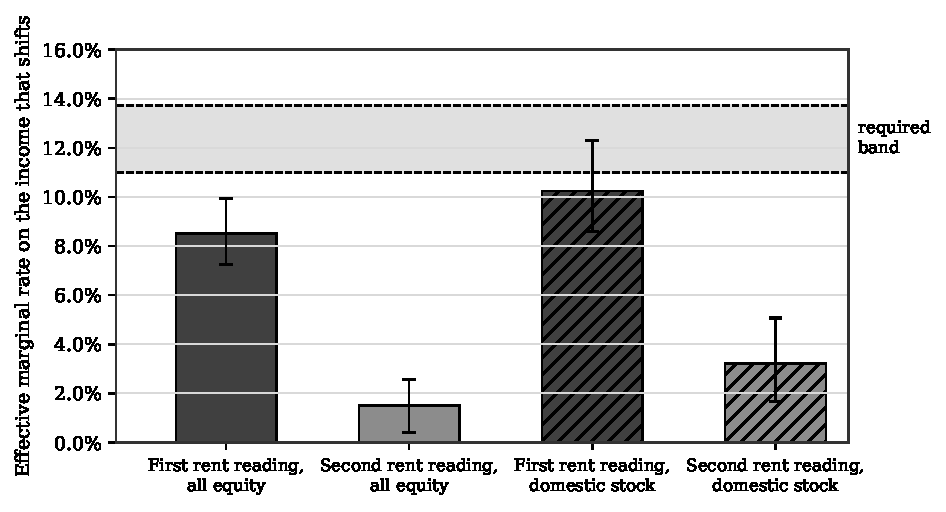
\includegraphics[width=0.84\textwidth]{fig3_capital_tax.pdf}
\caption{The assembled effective marginal rate on income that moves from wages to AI capital,
against the rate required to replace the wage taxes lost. Bars are central values, whiskers the
fifth to ninety-fifth percentile of the swept components; the shaded band is the required rate
across the two readings of the labor tax rate. The two left bars use the taxable-holder share
measured over all equity outstanding, the two right bars the same numerator over domestically held
stock. Scenario, on a construction reproduced by independent rebuild.}
\label{fig:tauk}
\end{figure}

\subsection{What would have to be true for the conclusion to reverse}

A shortfall is only interesting if it survives the assumptions that would close it, so we apply
each of those in turn and then together, all on the all-government version for comparability.
Treating the foreign-held share of equity as bearing a fifteen percent treaty withholding rate at
the owner level, rather than nothing, raises the assembled rate to \result{TauKWithholding}
percent; that treaty rate is a stated assumption and not a measurement. Taking the debt-financed
share from the filers' own books rather than the economy-wide stock ratio raises it to
\result{TauKLowDebtShare} percent, because the debt-financed term is negative. Applying both
together gives \result{TauKJointWeakening} percent, still below the required
\result{RequiredAllGovEasy} percent. The second rent reading moves in the opposite direction, to
\result{TauKKN} percent.

One further assumption works in the paper's favor and belongs here for that reason. The labor
tax rate is economy-wide, while displacement is not uniform across the wage distribution. Using
the payroll and income tax rates by wage quintile already in the release, the effective rate runs
from \result{LaborTaxQuintileLow} percent at the bottom to \result{LaborTaxQuintileHigh} percent
at the top, so displacement concentrated in the bottom quintile would require only
\result{RequiredBottomQuintile} percent rather than \result{RequiredTopQuintile} percent at the
top. Even that lower requirement is above the assembled rate on either jurisdiction.

\subsection{Pass-through, and what it can do to the comparison}

The condition in Definition~\ref{def:condition} carries a coefficient that the headline comparison
sets to one. Written as $\tau_k \ge \tau_\ell (1 - R)$, it assumes that every dollar of displaced
wages reappears as a dollar of taxable US capital income. Making that explicit,
\begin{equation}
\tau_k \, g \;\ge\; \tau_\ell\,(1 - R), \qquad
\tau_k^{\ast} = \frac{\tau_\ell\,(1 - R)}{g},
\label{eq:passthrough}
\end{equation}
with $g$ the taxable US capital income generated per dollar of displaced wages, bounded in
$[0,1]$ with output preserved. Everything reported above is the case $g = 1$, and it stays the
headline because $g$ cannot be sourced. Incomplete pass-through can only widen the shortfall,
never close it: any $g$ below one raises the required rate, and the decomposition of a displaced
wage dollar in Appendix~\ref{app:detail}, which puts $g$ at \result{GLow} to \result{GHigh}, is
scenario arithmetic reported there for that reason.

\subsection{The boundary, and what would have to happen for the condition to close}

The bound $g \le 1$ belongs to the output-preserved case. If AI raises output, a displaced wage
dollar can be associated with more than a dollar of taxable capital income, and $g$ can exceed
one. Stating the condition that way turns a comparison of point estimates into a boundary, which
is the more useful object: Figure~\ref{fig:boundary} draws the fiscal balance
$\tau_k \, g - \tau_\ell (1 - R)$ over the retained wage share and $g$, with the zero contour for
each jurisdiction and each labor tax reading.

Two things can be read straight off it. At the measured retained wage share, the condition closes
only if $g$ reaches \result{GStarFedEasy} to \result{GStarFedHard} on the federal-only version,
or \result{GStarAllEasy} to \result{GStarAllHard} on the all-government one. Every one of those
is above the output-preserved ceiling, so with output preserved the condition does not close at
the assembled rate anywhere on the grid. And the conclusion reverses only in the upper region:
either output rises enough to carry $g$ well past one, or the share of displaced wages that comes
back as wages rises far above what the displaced worker data show.

\begin{figure}[htbp]
\centering
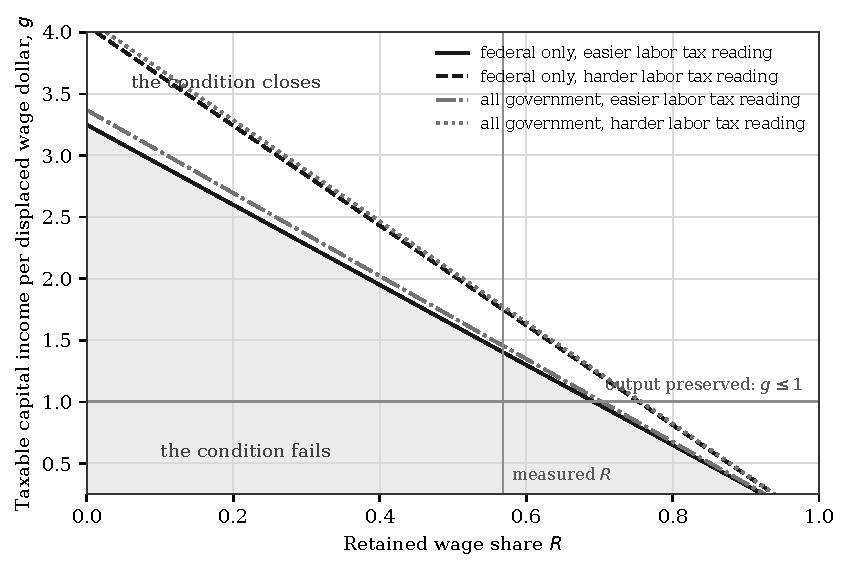
\includegraphics[width=0.84\textwidth]{fig6_boundary.pdf}
\caption{The fiscal balance per displaced wage dollar, $\tau_k \, g - \tau_\ell (1 - R)$, over the
retained wage share $R$ and the taxable capital income generated per displaced wage dollar $g$.
Each line is the zero contour for one jurisdiction and one labor tax reading, at the assembled
capital rate for that jurisdiction; the condition closes above a line and fails below it. The
shaded region is where it fails on the headline federal-only version. The horizontal line is the
output-preserved ceiling and the vertical line the measured retained wage share. Scenario, on the
assembled rate.}
\label{fig:boundary}
\end{figure}

\subsection{What the rate is a statement about}

Under full expensing the deduction precedes the income. The rate assembled here is therefore a
present-value wedge over the life of one marginal investment, while the replacement question asks
about tax collected in a year. The two are comparable only under three conditions: investment
constant, so that this year's deduction matches the deductions behind the income now taxed; rates
constant, so that the wedge on a project placed today is the wedge that applied to projects
already in place; and the capital stock stationary, so that both annual flows are steady. Under
those conditions the annual rate and the marginal wedge stand in the same ratio, and outside them
every comparison in this section fails. The transition runs against the paper rather than for it:
while investment grows, current deductions exceed the tax on income from a smaller earlier capital
stock, so revenue actually collected is below the assembled rate implies, and
Appendix~\ref{app:detail} sizes that with an illustrative path.

\subsection{Why the rate is low, and ownership matters more than profit shifting}
\label{sec:levers}

The binding constraint is who owns the claims. About \result{ThetaUntaxable} percent of US
corporate equity is held in forms the individual income tax barely reaches, chiefly retirement
accounts, foreign investors and nonprofits, leaving \result{ThetaTaxable} percent in taxable
accounts across a sourced range of \result{ThetaTaxableLow} to \result{ThetaTaxableHigh} percent
\citep{RosenthalAustin2016,RosenthalBurke2020,RosenthalMucciolo2024}. Of the gains that do accrue
there, \result{GainsUntaxedAtDeath} percent are held until death and never taxed, on 2014 data
\citep{CBO2014}, and what is realized is realized late, deferral cutting the present value by a
factor of \result{DeferralLow} to \result{DeferralHigh} on the later CRS estimates
\citep{Gravelle2022}. The two vintages are a decade apart and agree that roughly half of accrued
gains never bear tax, which is why we carry both rather than the newer alone. The debt side has the same
structure: \result{InterestSheltered} percent of corporate interest goes to holders who do not pay
tax on it and \result{BondsRestOfWorld} percent of corporate bonds are held abroad. Together these
are why the owner's layer adds only \result{ShareholderLayerPct} percent to the rate on rents.

Profit shifting is real. How much it matters is a different question from how uncertain it is,
and the two are easy to conflate.

\paragraph{Sensitivity is not importance, and the lever table measures sensitivity.}
Table~\ref{tab:levers} moves each component across its range with the others held at central
values. That reports how much the answer would move if we were wrong about a parameter. It does
not report how much that channel reduces the rate. A parameter pinned to a narrow range by good
evidence has a small swing and may still be the largest determinant of the level, which is
exactly the argument Appendix~\ref{app:detail} already makes about the taxable-holder share. The
same logic applies to every row, so the table is reported here as an uncertainty diagnostic and
no claim about relative importance is drawn from it.

\paragraph{The counterfactual comparison, by mechanism rather than by package.} To ask which
channel matters we set each to its no-friction value and measure what happens to the level.
Ownership is not one mechanism but two, the share of equity held in taxable accounts and the
deferral and step-up that erode what reaches those accounts, and bundling them would overstate
the comparison. They are kept apart.

\begin{table}[htbp]
\centering
\caption{Counterfactual contribution of each mechanism to the assembled marginal rate,
federal-only basis, Barkai rent reading. ``Alone'' sets that mechanism to its no-friction value
with the others at sourced centrals. The Shapley column averages each mechanism's marginal
contribution over all six orders of removal and sums exactly to the joint effect. Scenario.}
\label{tab:counterfactual}
\begin{tabular}{lrr}
\toprule
Mechanism set to its no-friction value & Alone & Shapley \\
\midrule
Taxable shareholder base complete & \result{ShThetaAlone} & \result{ShThetaShapley} \\
Deferral and step-up eliminated & \result{ShDeferAlone} & \result{ShDeferShapley} \\
Profit shifting eliminated & \result{ShShiftAlone} & \result{ShShiftShapley} \\
\midrule
All three together & & \result{ShJoint} \\
\bottomrule
\end{tabular}
\end{table}

Read alone, the three are closer than a bundled comparison suggests. Eliminating profit shifting
adds \result{ShShiftAlone} percentage points and eliminating deferral adds
\result{ShDeferAlone}, which is larger but not by much. The taxable shareholder base is the
outlier at \result{ShThetaAlone}.

The alone column understates the ownership mechanisms because they are complements: fixing
deferral makes the taxable base matter more and the reverse. The Shapley attribution, which
averages over every order of removal and sums exactly to the joint effect of
\result{ShJoint} points, puts the taxable base at \result{ShThetaShapley}, deferral at
\result{ShDeferShapley} and profit shifting at \result{ShShiftShapley}.

So the comparison the title draws is this one. The single largest mechanism, the taxable
shareholder base, is about \result{ShRatioTheta} times profit shifting. The two ownership
mechanisms together are about \result{ShRatioPair} times it, and that figure is a package and is
labelled as one. What does not hold is a claim that every ownership mechanism individually dwarfs
shifting: deferral does not.

Neither counterfactual is a policy. No reform abolishes profit shifting or places all equity in
taxable hands with no deferral, so the rows bound what each mechanism can contribute rather than
proposing anything.

Under the Karabarbounis and Neiman rent reading profit shifting contributes exactly nothing, and
that follows from the model rather than from the data: shifting operates only on the rent
component and that reading sets the rent share to zero. It is reported for completeness and
carries no evidential weight in the comparison.

\paragraph{The denominator caveat, which runs against us.} Both sources for the shifted share
measure a share of \emph{foreign} profits, while the assembly applies the parameter to the whole
rent base, treating a dollar of US rent as booked abroad with that probability. That overstates
shifting unless essentially all rent is earned through foreign affiliates. Correcting it would
raise the assembled rate and narrow the shortfall this paper reports, and it would also
\emph{shrink} the profit-shifting counterfactual above, which is the direction that strengthens
the comparison rather than the paper's headline. It is stated at L11 in
Section~\ref{sec:limitations} and bounded there.
\begin{table}[htbp]
\centering
\caption{The levers, ranked by sensitivity to parameter uncertainty rather than by importance.
Each is moved across its whole sourced or swept range with the others at central values, so a row
reports how much the answer would move if we were wrong about that parameter, not how much the
channel reduces the rate. For the latter see Table~\ref{tab:counterfactual}. Scenario.}
\label{tab:levers}
\input{tables/tab_levers.tex}
\end{table}


\paragraph{The separate checks are not cumulative, so here they are jointly.} This paper carries
two parameters that move the answer in the paper's own favour when they move: the retained wage
share $R$, whose specifications span \result{RSensLow} to \result{RSensHigh} and which lowers the
required rate as it rises, and the foreign-rent share $\phi$ of
Section~\ref{sec:limitations}, which raises the assembled rate as it falls. Checking them one at
a time and reporting both as though the checks accumulated would be a mistake, because the favourable ends compound.

\begin{table}[htbp]
\centering
\caption{The replacement condition over the retained wage share and the foreign-rent share
jointly, federal-only basis, narrower labor tax reading. Cells are the assembled rate less the
required rate in percentage points; negative is a shortfall. Scenario.}
\label{tab:joint}
\begin{tabular}{lrrrr}
\toprule
 & assembled rate & $R=0.568$ & $R=0.600$ & $R=0.637$ \\
\midrule
$\phi = 1.00$ & 7.75 & $-3.26$ & $-2.45$ & $-1.50$ \\
$\phi = 0.60$ & 8.30 & $-2.71$ & $-1.90$ & $-0.96$ \\
$\phi = 0.30$ & 8.71 & $-2.30$ & $-1.49$ & $-0.54$ \\
$\phi = 0.00$ & 9.13 & $-1.89$ & $-1.08$ & $-0.13$ \\
\bottomrule
\end{tabular}
\end{table}

The condition closes in \result{JointClosing} of the \result{JointCells} cells, so the direction
survives the joint move. The margin does not. At the corner most favourable to us, $\phi = 0$ and
$R = \result{RSensHigh}$, the shortfall is \result{JointNarrowest} percentage points against
\result{JointWidest} at the central case. That is close enough to nothing that we will not claim
the shortfall is established at that corner, only that it has not reversed anywhere on the grid.

Two things follow and both weaken the paper rather than strengthen it. The headline shortfall of
\result{JointWidest} points is a central-case figure and not a lower bound. And a reader who
holds different views about $R$ and $\phi$ than we do can reach a near-tie without leaving the
range either parameter is defensibly in. The result we are willing to defend is the sign across
this grid, not the size at any point in it.

\subsection{Checks, and what this module does not reach}

Two published figures check the assembly and one limitation runs against our own finding; both are set out in Appendix~\ref{app:detail}. In short, our shareholder layer corroborates the Congressional Research Service's text figure once the two are put on a common base, and the base construction treats foreign holders as bearing no tax at the owner level though dividends to them bear withholding tax. That effect is sized in Section~\ref{sec:fiscal} above: at a fifteen percent treaty rate it raises the assembled rate to \result{TauKWithholding} percent, and to \result{TauKJointWeakening} percent with the filers' own debt share as well, both below the \result{RequiredAllGovEasy} percent the condition requires. What stays open is the actual effective withholding rate, which varies by treaty and with the split between dividends, which bear it, and capital gains realized by foreign holders, which generally do not.


\section{The household counterpart: ownership without access}
\label{sec:household}

The revenue side of the condition fails because of who owns the corporate claims. This
section asks whether the same ownership structure governs the household side, measured on
survey microdata rather than on tax components. It does, and the mechanism is the same.

\subsection{Whose capacity falls}

In the Survey of Consumer Finances we move a share of aggregate wage income to capital
income, distribute it by actual ownership and hold debts fixed: incidence under stated
conventions, not a forecast. With payments fixed, a household's burden rises exactly when
its income falls.

Three results hold across the conventions we varied. Capacity falls for about \result{HHBottomQuartileAffected} percent
of bottom-wealth-quartile households against about \result{HHTopOnePctAffected} percent of
the top one percent, monotone in wealth. About three fifths of household debt is owed by
households earning more from wages than they hold in capital, at any size of shift. And
broadened ownership through retirement vehicles moves nothing unless the holdings can be
spent, because ownership without access cannot service a payment:
\result{HHEquityOutsideHouseholds} percent of corporate equity sits outside the household
sector, another \result{HHEquityInRetirement} percent in retirement vehicles.

The fiscal condition falls short on a rate, which a legislature can change; this one on who
holds the capital, which a rate does not. Closing the whole fiscal gap and distributing it
per capita moves household capacity little.

Illustrative only, and post hoc: for the median dollar of affected debt, restoring capacity
takes roughly \result{HHRestoreFive} percent cumulative real growth at a five percent shift,
\result{HHRestoreTen} percent at ten. Median and upper quartile are stable across the 2019
and 2022 waves; the lower quartile is not. The pre-specified boundary is a maximum set by
one household and is not reported. Nor are the policy arrangements, since one statistic
counts households crossing a line and the other conditions on a group the policy changes,
nor the holder mapping, which moves sevenfold with the agency classification. It is neither
the debt-service stress test of \citet{BartscherKuhnSchularickSteins2020} nor the
model-based growth threshold of \citet{Bayraktar2026}.

\subsection{Exposure type is a pay effect, and how displacement arrives changes who pays}

Households whose earners are physically exposed look more fragile than those whose earners are
cognitively exposed, and that difference does not survive a control for pay: reweighting either
group to the other's pay distribution leaves \result{PayGapSurvivingLow} to
\result{PayGapSurvivingHigh} percent of the raw gap, and on one index and one survey the contrast
reverses sign. Exposure type is largely a proxy for pay here, and the direction, confirmed by the
rebuild, is what we report.




\section{If AI fails}
\label{sec:bust}

This module prices the opposite direction through the same engine as the displacement case, so
that the asymmetry in the central claim is not an artifact of having stress-tested only one
outcome. An AI bust turns out to be a large fiscal event and a small credit event, which inverts
the displacement case.

\subsection{What the AI side is financed with, in bounds}

Any claim about a bust depends on how the investment was financed, so the AI side is reported as
bounds by tier in Table~
ef{tab:aitiers}: a measured tier of on-balance-sheet debt from nine named registrants, a verified secondary tier of large bank commitments to AI-adjacent industries, a scenario tier for AI-attributable equity, and an unsourced tier of off-balance-sheet vehicles and hardware-backed lending that contributes nothing to the total. Inside the
measured tier the nine filers fund capital spending largely from operating cash flow, a
self-funding ratio of \result{SelfFunding} and a debt-financed share of
\result{DebtFinancedShare} percent; Appendix~\ref{app:detail} gives the levels and the drawn
portion of the bank commitments, and the fourth tier, which \citet{BIS2026} describes as dominant,
is not sourced at all.

\begin{table}[htbp]
\centering
\caption{The AI side by tier of evidence. Tier 1 is measured from filings and is a lower bound on
the total; tier 4 is unsourced and is the hole the financing verdict turns on. Cells with no
sourced value read n/a.}
\label{tab:aitiers}
\input{tables/tab_ai_tiers.tex}
\end{table}

\subsection{The financing verdict, which is conditional}

Two historical patterns bracket a bust of this kind, with different fiscal consequences. In the
equity-led case of 2000 to 2002 federal receipts fell \result{EquityLedReceiptsPct} percent and
corporate tax \result{EquityLedCorpPct} percent; in the debt-led case of 2007 to 2009 receipts
fell \result{CreditLedReceiptsPct} percent and corporate tax \result{CreditLedCorpPct} percent.
Both are verified from published aggregates.

On the nine filers' own books the structure sits near the equity-led pattern, and stopping there
would be wrong. The verdict leaves that pattern on \result{FlipToBetweenBn} billion dollars of
additional debt-financed capital spending, \result{FlipToBetweenShare} percent of the tier 2
commitments, and reaches the debt-led pattern on \result{FlipToDebtLedBn} billion,
\result{FlipToDebtLedShare} percent of them. The drawn portion alone already exceeds the first
threshold, and tier 4 is unmeasured.

\begin{quote}
The defensible statement is that on the nine filers' own balance sheets the structure resembles
the equity-led case. The statement that the structure resembles the equity-led case is not
defensible, and we do not make it.
\end{quote}

\subsection{The bust through the same engine}

Converted to a wage-bill equivalent, a bust costs \result{BustWageLow} to \result{BustWageHigh}
percent of the wage bill, \result{BustRatioLow} to \result{BustRatioHigh} times smaller than the
ten percent displacement case. Household credit losses are \result{BustCreditLow} to
\result{BustCreditHigh} billion dollars, and output falls \result{BustGDPLow} to
\result{BustGDPHigh} percent, well inside the supervisory severely adverse scenario. Federal
receipts, by contrast, fall \result{BustReceiptsLow} to \result{BustReceiptsHigh} billion dollars
on the verified historical episodes: an order of magnitude larger than the terminal-year fiscal
loss at ten percent displacement, and arriving through capital gains and corporate receipts rather
than wage taxes. These are scenario figures.

Why the bust transmits so weakly to households is measured, and it is the ownership fact that drove
Section~\ref{sec:fiscal}: the top one percent of households hold \result{TopOnePctEquity} percent
of corporate equity and the bottom half \result{BottomHalfEquity} percent \citep{FRBDFA}, so a
fall in equity value lands where the propensity to consume out of wealth is lowest,
\result{MPCWealth} cents in the dollar per year \citep{ChodorowReichNenovSimsek2021}. The
concentration that makes the capital tax base hard to reach makes the wealth channel weak. Two
caveats: that propensity is sourced and checked against two episodes rather than estimated here,
and the output path does not feed bank-channel damage back into itself.

\subsection{Composition, and why we do not net the two sides}

A reader will want a single number per holder: what it gains or loses across the two states.
Netting requires a dollar base on each side, and the AI side has none, so the holder comparison has to stay a contrast in composition rather than a net position, and this section adds nothing to it.

One consequence of that point matters for the federal row. A
composition contrast scored on holdings cannot see a tax claim at all, and the state's claim on AI
capital income is fiscal rather than proprietary: it is the capital tax of
Section~\ref{sec:fiscal}. Federal receipts fall \result{BustReceiptsLow} to
\result{BustReceiptsHigh} billion dollars if AI capital income falls, and none of that appears in
a holdings comparison.

\subsection{Two directions, two tax bases}

The instruments that would protect against the two failure directions are nearly disjoint, but not
because a bust leaves the wage side untouched. It touches it, by the amount reported above, and
the point is that it reaches the wage side through a channel one to two orders of magnitude
smaller than displacement does while reaching the federal budget through a different tax base
entirely. The federal government is fiscally exposed in both states, through different tax bases,
and instruments that protect one base do not protect the other.

The rate itself links the two states. Revenue at risk in a bust is linear in the capital tax rate,
so a rate set high enough to close the displacement-side condition, a multiple of
\result{ClosingMultipleLow} to \result{ClosingMultipleHigh} on the assembled rate, puts the same
multiple of capital-linked revenue at risk in a bust. The ratio of bust exposure to success-state
revenue does not depend on the rate at all, so raising it scales both sides of the state's
position together rather than tilting one against the other. Whether the level effect is large
cannot be settled here: it requires a measure of US AI capital income, and no such measure exists
in our data.


\section{Implications for Individuals, Organizations, and Society}
\label{sec:implications}

A measured rate is only useful if it changes what somebody does, and the measurement here is
that no revenue shortfall is established on either tax object. This section says what
follows for the people a labor-to-capital shift reaches, for the organizations that would have
to act, and for the public interest. We mark what the evidence supports and what it does not,
because the gap we measure is large enough to invite recommendations it cannot carry.

\paragraph{For the people a shift reaches.} The household result is the one with the most direct
bearing on individuals, and it is unwelcome. Capacity to service existing debt falls for about
\result{HHBottomQuartileAffected} percent of bottom-wealth-quartile households against about
\result{HHTopOnePctAffected} percent of the top one percent, monotone in wealth. The reason is
not complicated: the households that owe the debt are not the households that own the equity, and
contracts do not move when factor shares do. A payment fixed in nominal terms becomes harder to
meet exactly when the income behind it falls.

The remedy that suggests itself, giving households a share of the capital, does not work in the
form usually proposed. Broadening ownership through retirement vehicles moves the boundary by
exactly zero unless the holdings can be spent, because ownership without access cannot service a
payment. For the individual at the point of decision this is the practical statement: a
retirement account is not a buffer, and policy that treats broadened ownership as though it were
one will not reach the person whose payment is due this month. Access, not ownership, is the
operative variable.

\paragraph{For managers and organizations.} The conclusion for anyone planning around a capital
tax instrument is that the instrument is weaker than its headline rate suggests, and weak for
structural reasons that will not be fixed by a rate change. An organization modeling its own
exposure to a tax rise on capital income should model the owner layer explicitly rather than
applying a statutory rate, because the owner layer adds only \result{ShareholderLayerPct} percent
to the rate on rents at central values.

There is a timing point as well, and it runs against the optimistic reading. Under full expensing
the deduction precedes the income, so while investment is growing, current deductions exceed the
tax on income from a smaller earlier capital stock. Revenue actually collected during an
investment boom is below what the assembled rate implies, not above it. Any plan that counts on
the boom paying for the transition has the sign wrong.

\paragraph{Strategic implications.} The ownership finding reframes a debate that has been
conducted largely in terms of enforcement. If the binding constraint were profit shifting, the
instruments would be information exchange, transfer pricing rules and minimum taxes, and the
problem would be one of administrative capacity. Our ranking says the constraint is third on that
list. The instruments that actually move the rate are the ones that touch deferral, step-up at
death and the boundary of the taxable shareholder base, which are domestic, legislative and
politically harder, and which have had a fraction of the attention.

The second strategic point is about hedging, and it cuts against the state's own position. The
rate links the two directions of risk without trading one against the other: revenue at risk in a
bust is linear in the capital tax rate, so raising the rate enough to close the displacement-side
condition scales bust-state exposure by the same multiple. A government cannot tax its way out of
one direction without increasing what it loses in the other. That is an argument for instruments
that are not rates at all, and we say so without claiming to know which.

\paragraph{For society and equity.} The same concentration of ownership runs through every result
in this paper, and its distributional reading is blunt. The capital tax reaches little because
most corporate claims sit where the income tax does not. Households cannot be made whole by
ownership because most corporate equity is not theirs and what is theirs cannot be spent. A bust
transmits weakly to households because the assets that fall are held by the households least
likely to change their spending. One fact about who owns American corporate capital explains a
revenue problem, an incidence problem and a transmission result.

That is a statement about the structure of claims, not about anybody's deserts, and we draw one
narrow conclusion from it. A shift of income from labor to capital is not distributionally
neutral and cannot be made so by adjusting a rate after the fact, because the rate operates on a
base that most households are not in. Whether to act on that, and how, is a question for a
legislature. What the measurement supplies is the constraint any answer has to satisfy, and the
knowledge that the obvious answers, a higher rate and broader nominal ownership, do not satisfy
it.


\section{Limitations}
\label{sec:limitations}

Every limitation below is numbered so that the avenues in Section~\ref{sec:future} pair with it
one to one. Several of them run against our own finding, and those are stated first.

\paragraph{L1. Three components are swept rather than sourced.} The assembled rate is a scenario
in the strict sense. Three of its components have no single sourced value and are drawn
uniformly over stated ranges, so the central figure is a point inside a grid rather than an
estimate with a sampling distribution. We report the share of that grid in which the condition
closes, \result{PassShareOursEasy} percent against the easier labour tax reading on our base, and
state plainly that a share of a uniformly weighted grid is not a probability. The corners of the
space reach further than the pass shares suggest: the analytic maximum on our base is
\result{AnalyticMaxOurs} percent, which exceeds the easier required rate, which is why the claim
this paper makes is about the share of the space rather than about every corner of it.

\paragraph{L2. The base of the taxable shareholder share is load-bearing and contestable.} Ours
is equity in taxable accounts over all US equity outstanding; the Congressional Research Service
uses the same numerator over domestically held stock alone. Ours is the right base for a rate on
a dollar of US surplus whoever holds it, because a foreign holder bears close to no US tax at the
owner level and that dollar is still in the surplus. The choice matters: on the domestic-holder
base the central rate rises to \result{TauKCRSCentral} percent and the share of the grid in which
the condition closes rises to \result{PassShareCRSEasy} percent. The central case falls short on
either base, but how far short depends on the choice, and we report both rather than only ours.

\paragraph{L3. Foreign holders are treated as untaxed at the owner level.} The base construction
treats dividends to foreign holders as bearing no US tax at the owner level, though they bear
withholding tax at treaty rates. Applying a fifteen percent treaty rate raises the assembled rate
to \result{TauKWithholding} percent, and to \result{TauKJointWeakening} percent together with the
filers' own debt share, both still below what the condition requires. The treaty rate is a stated
assumption rather than a measurement, and the effective rate actually borne, which varies by
treaty and with the split between dividends and capital gains realized by foreign holders,
remains open.

\paragraph{L4. The assembled rate is a marginal wedge and the question is about annual revenue.}
Under full expensing the deduction precedes the income, so the rate assembled here is a
present-value wedge over the life of one marginal investment, while replacement asks about tax
collected in a year. The two are comparable only if investment is constant, rates are constant
and the capital stock is stationary. Outside those conditions every comparison in
Section~\ref{sec:fiscal} fails. The transition runs against this paper rather than for it, since
revenue actually collected during an investment boom is below what the assembled rate implies,
but we have not bounded the size of that effect beyond the illustrative path in
Appendix~\ref{app:detail}.

\paragraph{L5. The effective labour tax rate does not vary across the wage distribution.} It is a
single economy-wide rate, and because displacement is concentrated away from the top of the
distribution a flat rate probably overstates the revenue loss from displacing low-paid workers
and understates it from displacing high-paid ones. Using rates by quintile, displacement
concentrated at the bottom would require \result{RequiredBottomQuintile} percent rather than
\result{RequiredTopQuintile} percent at the top. Even that lower requirement exceeds the
assembled rate on either jurisdiction, so the direction is known while the net effect is neither
signed nor bounded.

\paragraph{L6. The pass-through coefficient cannot be sourced.} The boundary in
Section~\ref{sec:fiscal} is drawn over a coefficient for which we have no verified estimate here
or, so far as we located, anywhere. The headline sets it to one and the appendix sweeps it, and
the sweep is the weakest arithmetic in the paper. Its only purpose is directional: incomplete
pass-through can only widen the shortfall, never close it.

\paragraph{L7. The household result is incidence arithmetic, not a forecast.} We move a share of
aggregate wage income to capital income, distribute it by actual ownership and hold debts fixed.
That is incidence under stated conventions. It is not a prediction, not a causal estimate, and
not a general-equilibrium result, and the households it describes would in reality adjust in ways
the arithmetic does not represent.

\paragraph{L8. The classification of the housing agencies moves the holder mapping sevenfold.}
Of the debt owed by households whose capacity falls, the share the federal government holds or
guarantees moves by a factor of about seven between the central classification and the
alternative agency treatment. That is the largest single judgement call affecting the incidence
result, it is a classification choice rather than a measurement, and we have not resolved it.

\paragraph{L9. The bust direction rests on two historical episodes.} The fiscal consequence of a
bust is bracketed by the equity-led case of 2000 to 2002 and the debt-led case of 2007 to 2009,
both verified from published aggregates. Two episodes are not a distribution, the wealth effect
we apply is sourced rather than estimated here, and the output path does not feed bank-channel
damage back into itself.

\paragraph{L10. Off-balance-sheet financing is unmeasured, so the financing verdict is
conditional.} The measured tier is nine registrants' on-balance-sheet facts. Off-balance-sheet
vehicles, hardware-backed lending and securitization contribute nothing to it. The defensible
statement is that on the nine filers' own balance sheets the structure resembles the equity-led
case. The statement that the structure resembles the equity-led case is not defensible, and we do
not make it.


\section{Avenues for further research}
\label{sec:future}

Each avenue below addresses the limitation carrying the same number in
Section~\ref{sec:limitations}.

\begin{description}[leftmargin=2.4em,style=nextline]

  \item[FR1] Researchers should source the three swept components directly, the rent share from
  firm-level production data, the deferral factor from realization histories and the debt share
  from a marginal rather than a stock ratio, which would replace the swept grid with an estimate
  carrying a sampling distribution and turn our share of a space into a confidence statement.

  \item[FR2] Researchers should construct both bases for the taxable shareholder share from the
  same underlying holder data and report the assembled rate on each, rather than taking one base
  from one literature and comparing it with a figure built on the other, which is the comparison
  our own published check had to be corrected for.

  \item[FR3] Researchers should measure the effective withholding rate actually borne by foreign
  holders treaty by treaty, and separate dividends, which bear withholding, from capital gains
  realized by foreign holders, which generally do not. That would replace the single stated
  treaty rate with a measured one and close the largest open assumption in the base construction.

  \item[FR4] Researchers should build an annual-revenue counterpart to the marginal wedge, using
  an investment path and a capital stock rather than a single marginal project, so the quantity
  compared against a replacement requirement is the quantity a budget actually collects. Our
  illustrative path shows the mechanism and does not size it.

  \item[FR5] Researchers should replace the single economy-wide labour tax rate with rates by
  position in the income distribution, and pair them with an assumed incidence of displacement
  across that distribution, which would sign and bound an effect we can currently only describe.

  \item[FR6] Researchers should estimate the pass-through coefficient directly, measuring how
  much taxable domestic capital income a dollar of displaced wages actually generates, which is
  the single input that would convert our boundary from a surface into a located point. We
  located no estimate of it anywhere, which may itself be the finding.

  \item[FR7] Researchers should embed the incidence arithmetic in a model that lets households
  adjust, so the measured boundary can be compared against a behavioural one and the difference
  attributed. \citet{Bayraktar2026} supplies one such model and the comparison has not been made.

  \item[FR8] Researchers should resolve the housing agency classification against the legal and
  budgetary treatment of conservatorship rather than reporting both readings, which would remove
  the factor-of-seven swing that is currently the largest unresolved judgement in the incidence
  result.

  \item[FR9] Researchers should extend the bust bracket beyond two US episodes, using
  international equity busts with comparable fiscal detail, and should estimate the wealth effect
  on the relevant population rather than importing a sourced average.

  \item[FR10] Researchers should build the off-balance-sheet side of the capital stock from
  securitization prospectuses, vehicle-level filings and supervisory data on lending secured
  against computing hardware, which would make the financing verdict unconditional rather than
  restricted to what nine balance sheets disclose.

\end{description}


\section{Conclusion}
\label{sec:conclusion}

If income moves from labour to capital, the tax system has to collect on the second what it loses
on the first. We stated that requirement as a condition, assembled both of its sides from sourced
components, and measured how far the existing system falls short.

On a consistently federal basis the effective marginal rate on income shifting from wages to
capital is \result{TauKFederalOnly} percent, against the \result{RequiredFedEasy} to
\result{RequiredFedHard} percent replacement requires. Written with an explicit pass-through
coefficient, the comparison becomes a boundary, and the boundary is the more useful object: the
condition closes only where taxable capital income per displaced wage dollar reaches
\result{GStarFedEasy} to \result{GStarFedHard}, above the ceiling of one that output-preserving
displacement implies. Making the comparison consistent across jurisdictions widens the gap rather
than closing it, because the state adds more to the labour side than to the capital side.

The reason the rate is low is the contribution. It is not profit shifting, which ranks third of
seven levers and moves the assembled rate by \result{SwingShifted} across its entire range,
against \result{SwingDeferral} for deferral and step-up at death. What binds is ownership. About
\result{ThetaUntaxable} percent of US corporate equity sits in forms the individual income tax
barely reaches, and of the gains that do accrue in taxable accounts,
\result{GainsUntaxedAtDeath} percent are never taxed at all. A legislature can change a rate. It
cannot easily change who owns the claims, and the rate operates on a base most households are
not in.

That single fact does more work than one result. The same ownership concentration means
household debt-service capacity cannot be restored by broadening ownership, since
\result{HHEquityOutsideHouseholds} percent of corporate equity sits outside the household sector
and broadened ownership without liquidity moves the boundary by exactly zero. It means an equity
bust is a large fiscal event and a small credit event, because the assets that fall are held
where the propensity to consume is lowest. The revenue problem, the incidence problem and the
transmission result are three readings of one structural fact.

We do not claim this settles which tax base is right, and we state the case against our own
choice where it arises. Three components are swept rather than sourced, the pass-through
coefficient cannot be sourced at all, and the household figures are incidence arithmetic rather
than forecasts. What holds on every base and under every reading we can defend is that the
central case falls short, that the shortfall is governed by ownership rather than by enforcement,
and that the instruments which would actually move it are the ones that have had the least
attention.


\section*{Declarations}

\paragraph{Licence.} This preprint is posted under a Creative Commons Attribution 4.0
licence, under which the authors retain copyright and the work may be reused with
attribution. The replication package carries the same licence for its data artifacts and the
MIT licence for its code, so the posted version and the package do not carry conflicting
terms.

\paragraph{Data availability.} A replication package is supplied with this paper as
supplementary material. It contains the measured artifact behind every reported value, 55 JSON
and 49 CSV files, one per measured object, together with the code that turns them into the
tables, figures and in-text values: every \verb|\result| macro printed here resolves to a key
in that tree, so any number can be traced to a file. It does not contain the raw survey and
supervisory microdata, which are obtainable from the providers named in the data section but
are not ours to redistribute, so the package supports verification of every reported figure
from the processed artifacts and does not by itself support a rebuild from raw microdata. An
earlier version of this statement promised a private repository reachable through journal
review, which is not available to a reader of a preprint, and is replaced by the supplementary
package for that reason. The same tree is also public in a repository that carries the
generators, the pre-registrations and the rebuild records in addition to the artifacts, under
the MIT licence for code and Creative Commons Attribution 4.0 for data\ifanon; its address is
withheld here because it would identify the authors\else{} at
\url{https://github.com/MohitPratapSinghRathore/physical-ai}\fi. The corresponding author
will supply anything further on request. The swept ranges behind every scenario figure, and the grid over which the
condition is evaluated, are part of the package.

\ifanon
\else
\paragraph{Disclosure statement.} The authors report no conflict of interest.
\paragraph{Funding.} This research received no external funding.
\fi

\paragraph{Use of generative AI.} During the preparation of this manuscript the authors used a
generative AI tool to assist with language editing and refinement of the text. The authors
reviewed and edited all output and take full responsibility for the content of the paper.
Generative AI was not used to generate the study's data, which are the public statistical
releases and company filings named in Section~\ref{sec:data}, and no reported value originates in
a model's assertion: every number in the text and in the tables is generated by the measurement
pipeline described in the paper and archived in the replication package.


\appendix

\section{The independent computational rebuilds}
\label{app:rebuild}

Three rebuild rounds have been run against the measurements in this paper. Each was carried out by
a separate run with no access to the project's code, working from raw data and a published
specification, and scored against expected values fixed before the round began.

Round one established the protocol and produced no comparable values in several modules, because
the specification it worked from left definitions unstated. Round two scored
\result{RepTwoScored} quantities, \result{RepTwoSealed} of them against fixed expected values:
\result{RepTwoFivePct} came within five percent and \result{RepTwoTolerance} inside the stated
tolerance, while \result{RepTwoMismatch} did not match. The mismatches had six root causes, of
which the largest were an undefined universe for one household object, a class omitted because the
specification described the exclusion rule in prose without enumerating the classes, and a
Treasury level the rebuild could not know was the sum of two published series. Three of the five
quantities withdrawn from this paper were withdrawn as a direct result. Round three covered the
two constructions the earlier rounds had not reached, the debt-only ratio and the assembled
capital tax rate, and matched all \result{RepThreeSealed} quantities,
\result{RepThreeRounding} within rounding and the remainder inside tolerance. Its two
non-rounding matches were traced exactly: one to a central value taken at a range midpoint rather
than at the sourced point, which the paper now reports at the sourced point, and one to the
maximum of a finite sample over a seven-dimensional box, which is an extreme order statistic with
no stable value and is now reported as the analytic corner instead.

The blind was procedural rather than enforced. The rebuild ran on the same machine, with the file
of expected values reachable at a path the specification names; it was not attached to the request
and was reported unopened until the rebuild was final. The supporting evidence is internal and
circumstantial: most insufficiencies were written before the file was opened, several of the
mismatch causes were among them, and the rebuild declined to use coefficients the specification
had leaked. On that basis the paper claims that these quantities were independently rebuilt under
a reported blind protocol, and never that they were independently verified.


\section{Further detail}
\label{app:detail}

The material below was moved out of the body for length. Nothing in it is altered.

\subsection{Checks, and what this module does not reach}

\emph{Supporting Section~\ref{sec:fiscal}, on the published figures the assembled rate is checked against and the limitation that runs against our own finding.}

Our shareholder layer at central values, \result{ShareholderLayerPct} percent, corroborates the
Congressional Research Service's text figure of about \result{CRSTextFigure} percent for the
effective capital gains rate on corporate profits. It does not reproduce that report's published
band of \result{CRSBandLow} to \result{CRSBandHigh} percent as printed, and should not: the band
already carries a taxable-share adjustment over domestically held stock. Rescaled to a common base
it is \result{CRSRescaledLow} to \result{CRSRescaledHigh} percent, and our figure sits inside it.
We report the correction rather than the original comparison, because as first written our own
check failed against our own construction.

The base construction treats foreign holders as bearing no tax at the owner level, though
dividends to them bear US withholding tax at treaty rates. That effect is sized in
Section~\ref{sec:fiscal}: applying a fifteen percent treaty rate to the foreign-held share raises
the assembled rate to \result{TauKWithholding} percent, and to \result{TauKJointWeakening} percent
together with the filers' own debt share, both still below the \result{RequiredAllGovEasy} percent
the condition requires. The treaty rate is a stated assumption, not a measurement, and what stays
open is the effective rate actually borne, which varies by treaty and with the split between
dividends and capital gains realized by foreign holders. The debt share is an economy-wide stock ratio, \result{DebtShareLow} to
\result{DebtShareHigh} percent, standing in for a marginal flow; the evidence in
Section~\ref{sec:bust} points below that range, and because the debt-financed term is negative, a
lower debt share would raise the assembled rate.

\subsection{The pass-through decomposition}

\emph{Supporting Section~\ref{sec:fiscal}, on the taxable capital income generated per displaced wage dollar.}

Equation~\eqref{eq:passthrough} in Section~\ref{sec:fiscal} writes the condition with the
pass-through coefficient $g$ explicit; the headline sets $g = 1$ because $g$ cannot be sourced.
What follows is the sensitivity behind that choice, and its only purpose is to show the
direction: incomplete pass-through can only widen the gap on the marginal rate, never close it.

A displaced wage dollar splits into the cost of the AI capital and services that replace the work,
a share $c$, and the surplus the adopting firm keeps, $1 - c$. The second is the adopting firm's
capital income. Only the first is revenue to the suppliers of AI capital, and only there does our
decomposition of a dollar of AI capital spending apply: \result{CapexDomesticLabor} percent
domestic labor, which is already inside $\tau_\ell (1 - R)$ and must not be counted twice,
\result{CapexImported} percent imported and never entering the US tax base, and
\result{CapexDomesticSurplus} percent domestic producer surplus. So
$g = (1 - c) + c \, s$, with $s$ that surplus share. Taking $c = \result{CapitalCostShare}$
percent gives $g = \result{GCentral}$ and a required rate of \result{RequiredPTEasy} to
\result{RequiredPTHarder} percent, against \result{RequiredEasy} to \result{RequiredHard} at
$g = 1$; across the swept range of $c$, $g$ runs from \result{GLow} to \result{GHigh}.

A second channel is reported separately because it is a different mechanism. If a share of the
adopting firm's retained surplus is competed away to consumers in lower prices, it is never taxed
as capital income. At \result{PriceThrough} percent of the retained surplus, $g$ falls to
\result{GWithPrice} and the required rate rises to \result{RequiredPriceEasy} to
\result{RequiredPriceHarder} percent.

Three statements about this sensitivity, since it is the weakest thing in the section. It is
scenario arithmetic: $c$ has no verified estimate here or, so far as we located, anywhere, and the
shares behind $s$ are swept ranges rather than sourced values. It does not double count the
profit shifting already inside the assembled rate: the import share removed here is payment that
never enters the US base, while shifted profit does enter it and is taxed at the lower rate the
assembly already applies, and the one case where the two could touch, an intra-firm import priced
as a transfer, would make $g$ too low and so runs against this correction. And it changes what can
be said about the economy-wide rate only conditionally: at the central case of the base
construction, an economy-wide rate of twenty to twenty-two percent still clears the required band;
it stops clearing once a price pass-through term is added. That is a reason to report the two
terms separately, not to fold either into the headline.

\subsection{The transition path under expensing}

\emph{Supporting Section~\ref{sec:fiscal}, on revenue during an investment boom.}

While investment grows, current deductions exceed the tax on income from a capital stock built
when investment was smaller, so net revenue from the sector is below the steady-state figure and
can be negative. An illustrative path, using the tax parameters of Section~\ref{sec:fiscal} and a
geometric investment series that is chosen rather than estimated, makes the size of that visible:
with investment growing at \result{TransitionGrowthRate} percent a year, net entity-level tax is
negative at \result{TransitionYearFive} per unit of investment in year five and still negative in
year twenty-five, while at zero growth it turns positive in year
\result{TransitionPositiveYear}. That path illustrates a mechanism and is not a forecast of
revenue. The mechanism itself is not in doubt: during an investment boom the revenue actually
collected is lower than the assembled rate implies, not higher.

\subsection{The financing mix inside the measured tier}

\emph{Supporting Section~\ref{sec:bust}, on how the observed AI investment is funded.}

The nine filers report \result{FilerCapexBn} billion dollars of capital spending against
\result{FilerOCFBn} billion of operating cash flow, a self-funding ratio of
\result{SelfFunding}, and a debt-financed share of capital spending of
\result{DebtFinancedShare} percent on those books, which is a lower bound because financing held
off those balance sheets does not appear in it. Of the bank commitments in the second tier,
roughly \result{AIDrawnBn} billion appears drawn \citep{CohenKillenLau2026}.

\subsection{Reading the lever ranking}

\emph{Supporting Section~\ref{sec:fiscal}, on the table of levers.}

One line of Table~\ref{tab:levers} is easy to read backwards. The taxable-holder share appears
last, with a swing of \result{SwingTheta}, because it is pinned to a narrow sourced range and not
because it does not matter: it is the largest single determinant of the level of the assembled
rate and the smallest remaining source of uncertainty in it.


\bibliographystyle{apalike}
\bibliography{references}

\end{document}
